\documentclass{beamer}
\usepackage[english]{babel}
\usepackage[utf8]{inputenc} % allow utf-8 input
\usepackage[T1]{fontenc}    % use 8-bit T1 fonts
\usepackage{hyperref}       % hyperlinks
\usepackage{url}            % simple URL typesetting
\usepackage{booktabs}       % professional-quality tables
\usepackage{amsfonts}       % blackboard math symbols
\usepackage{nicefrac}       % compact symbols for 1/2, etc.
\usepackage{microtype}      % microtypography
\usepackage{xcolor}         % colors
\usepackage{lipsum}
\usepackage{amsmath}
\usepackage{setspace}
\usepackage{bbm}
\usepackage[commentsnumbered]{algorithm2e}
\usepackage{parskip}
\usepackage{graphicx}
\usepackage{caption}
\usepackage{subcaption}
\usepackage{soul,xcolor}

%general settings
\setstcolor{red}
\graphicspath{
  {../report/figures/active/neural/}
  {../report/figures/active/linear/}
  {../report/figures/other/}
  {../report/figures/online_similarity/neural/}
  {../report/figures/online_similarity/linear/}
}

%Information to be included in the title page:
\usetheme{Boadilla}
\usefonttheme[]{serif}
\title[Similarity Learning]{Active and Online Similarity Learning}
\subtitle[]{An application of bandits to Similarity learning}
\author[Ketan and Nicolas]{Ketan Jog and Nicolas Beltran}
\institute[]{Columbia University}
\date{May 2021}

\begin{document}

\begin{frame}
    \titlepage
\end{frame}


% ----------------------------------------------------
% General summary of accomplishments
% ----------------------------------------------------
\begin{frame}{}
\frametitle{What we did:}
Use bandit algorithms to solve the following problems:
\begin{itemize}
\item
    Online learning of a similarity measure.
\item
    Active learning of a similiarity measure (i.e. by querying labels).
\end{itemize}
\vspace*{1cm}
\begin{definition}
Similarity Measure: A function $\phi: \mathbb{R}^{2n} \to \mathbb{R}$ that maps datapoints $x, y \in \mathbb{R}^{n}$ to a real number in $\mathbb{R}$
according to how ``similar'' they are.
\end{definition}
\end{frame}


% ----------------------------------------------------
% Problem formulation
% ----------------------------------------------------
\begin{frame}{}
    \frametitle{Problem: Online Similarity Learning}
    At round $t$ the environment samples $K$ pairs of points $(x_{t,k}, y_{t,k}) \in \mathbb{R}^{2n}$.
    We choose pair $k_t \in [K]$ and get reward $r_{t,k_{t}} \in \{1, -1\}$ based on whether they are similar.

    We are trying to minimize:
    \[ R_T = \mathbb{E}\left[\sum_{t =1}^T r_{t, k^\star_t} - r_{t, k_t}\right] \]
    where $k_t^\star = \text{argmax}_{k\in [K]} \phi(x_{t,k}, y_{t,k})$
\end{frame}

\begin{frame}{}
    \frametitle{Problem: Active Similarity Learning}
    Learner has access to a dataset $D = \{x_i \in \mathbb{R}^n| i \in [N]\}$ of unlabeled points.
    The learner can query $T$ pairs of points in this set $D$ to obtain a dataset $D_T = \{(x_t, y_t, r_t) ~|  ~t \in [T]\}$.
    The learner mantains and estimate $\hat{\phi}_t \in \mathcal{F}$ of $\phi$, where $\mathcal{F}$ is its function class.
    Denote the loss between an estimate $\hat{\phi}$ a $\phi$ as
    \[ \mathcal{L}(\phi, \hat{\phi}) = \mathbb{E}_{(x, y) \sim \mathcal{D} \times \mathcal{D}}[(\hat{\phi}(x,y) - \phi(x, y))^2] \]
    Goal is to find
    \[\min_{\hat{\phi}_T \in \mathcal{F}} \mathcal{L}(\hat{\phi}_T, \phi)\]
\end{frame}

\begin{frame}{}
    \frametitle{First idea: Solution to online learning problem}
    Assume that
    \[\phi(x, y) = x^\top A y = \sum_{i =1}^n\sum_{j=1}^n x_i y_j A_{i,j} \]
    and then use linucb like methods.

    % two columns of pros and cons
    \vspace{1cm}
    \begin{columns}
        \begin{column}{0.5\textwidth}
            \textbf{Pros:}
            \begin{itemize}
                \item Easy to reason about.
                \item Fast.
            \end{itemize}
            \end{column}

            \begin{column}{0.5\textwidth}
            \textbf{Cons:}
            \begin{itemize}
                \item Can only learn linear similarities.
            \end{itemize}
            \end{column}
    \end{columns}
\end{frame}

\begin{frame}{}
    \frametitle{First idea Solution to online learning problem}
    {\small
    \begin{algorithm}[H]
        \setstretch{1}
          \SetKwInOut{Input}{Input}
          \Input{Rounds $T$ and exploration parameter $\alpha$}
          $A \gets I_{n^2}$\;
          $b \gets 0_{n^2}$\;
          \For{$t \in [T]$}{
            $\theta_t \gets A^{-1}b$\;
            Observe $K$ pairs of vectors $x^k \in \mathbb{R}^n$, $y^k \in \mathbb{R}^n$\;
            Create $z_{t,k} = (x_1^k, y_1^k, x_1^k, y_1^k, \dots, x_n^k y_{n-1}^k, x_n^k ,y_n^k)$\;
            \For{$k \in [K]$}{
              $p_{t,a} \gets \theta_t^\top z_{t,k} + \alpha \sqrt{z_{t,k}^\top A^{-1} z_{t,a}}$
            }
            Choose action $k_t = \text{argmax}_a p_{t,a}$ with ties broken arbitrarily\;
            Observe payoff $ r_t \in \{-1,1 \}$\;
            $A \gets A + z_{t,k_t}z_{t,k_t}^\top$\;
            $b \gets z_{t,k_t}r_t$\;
          }
        \caption{OnSim-LinUCB}\label{algo:active-linucb}

      \end{algorithm}
    }
\end{frame}

\begin{frame}{}
    \frametitle{Second idea: Solution to active learning problem}
    Use the ideas about optimist reward to encourage the learner to explore and chose points
    optimally.

    We replace
    \[ p_{t,a} \gets \theta_t^\top z_{t,k} + \alpha \sqrt{z_{t,k}^\top A^{-1} z_{t,a}} \]
    by
    \[ p_{t,a} \gets \sqrt{z_{t,k}^\top A^{-1} z_{t,a}} \]
\end{frame}

\begin{frame}{}
    \frametitle{Second Idea: Solution to active learning problem}
    {\small
    \begin{algorithm}[H]
        \setstretch{1.2}
          \SetKwInOut{Input}{Input}
          \Input{Rounds $T$ and exploration parameter $\alpha$}
          $A \gets I_{n^2}$\;
          $b \gets 0_{n^2}$\;
          \For{$t \in [T]$}{
            $\theta_t \gets A^{-1}b$
            Sample $K$ pairs of vectors $x^k \in R^n$, $y^k \in R^n$\;
            Create $z_{t,k} = (x_1^k y_1^k, x_1^k y_1^k, \dots, x_n^k y_{n-1}^k, x_n^k y_n^k)$\;
            \For{$k \in [K]$}{
              $p_{t,a} \gets  \alpha \sqrt{z_{t,k} A^{-1} x_{t,a}}$
                        }
            Choose action pair $k_t = \text{argmax}_ap_{t,a}$ with ties broken arbitrarily.\;
            Observe label $ r_t \in \{-1,1 \}$\;
            $A \gets A + z_{t,k_t}z_{t,k_t}^\top$\;
            $b \gets z_{t,j_t}r_t$\;
          }
          \caption{ActiveSim-LinUCB}
      \end{algorithm}
    }
\end{frame}


\begin{frame}{}
    \frametitle{More expressive model classes: Neural UCB}
    Method for solving the problem using a neural network to predict the rewards.
    \begin{itemize}
        \item Uses a Neural Network to model the rewards.
        \item Provably correct regret bound of $\tilde{O}(\tilde{d}\sqrt{T})$.
        \item Slow due to the computation of a very wide matrix.
    \end{itemize}
\end{frame}


\begin{frame}{}
    \frametitle{Second model}
    Assume that
    \[ \phi(x,y) = \cos\left(f(x;\mathbf{\theta}), f(y;\mathbf{\theta})\right) = \frac{\langle f(x;\mathbf{\theta}), f(y;\mathbf{\theta}) \rangle}{||f(x;\mathbf{\theta})||_2 ||f(y;\mathbf{\theta})||_2}\]
    or
    \[ \phi(x,y) = \langle f(x;\mathbf{\theta}), f(y;\mathbf{\theta}) \rangle \]
    where
    \[ f(x; \theta) = b_L + W_{L} \sigma\left(b_{L-1} +  W_{L-1} \sigma\left( \dots \sigma\left(b_1 + W_1 x\right)\right) \right)\]

    % two columns of pros and cons
    \vspace{1cm}
\end{frame}

\begin{frame}{}
    \frametitle{Algorithm for solving Online Similarity Learning Problem}
    {\footnotesize
    \begin{algorithm}[H]
        \setstretch{1.2}
          $A \gets I_{p}$\;
          \For{$t \in [T]$}{
            Observe $K$ pairs of vectors $x_t^k \in \mathbb{R}^n$, $y_t^k \in \mathbb{R^n}$\;
            \For{$k \in [K]$}{
              $p_{t,k} \gets \phi(x,y) + \alpha \sqrt{(\nabla_\theta \phi(x_t^k, y_t^k))^\top A^{-1}\nabla_\theta\phi(x_t^k,y_t^k)}$\;
            }
            Choose pair $k_t = \text{argmax}_k p_{t,k}$ with ties broken arbitrarily\;
            Observe payoff $ r_t \in \{-1,1 \}$\;
            \If{$t \mod \tau_r = 0$ }{
              $\theta \gets \text{Train}(\epsilon,E, \{(x_i^{k_i}, y_i^{k_i}, r_i)\}_{i=1}^t,b_s)$\;
            }
            \If{$t \mod \tau_T = 0$ }{
              $A \gets I_p$
            }
            $A \gets A + \nabla_\theta \phi(x_t^k, y_t^k)(\nabla_\theta\phi(x_t^k,y_t^k))^\top$\;
          }
          \caption{OnSim-NeuralUCB}\label{algo:onsim-neuralucb}
        \end{algorithm}
    }
\end{frame}

\begin{frame}{}
    \frametitle{Algorithm for solving Active Learning Problem}
    {\footnotesize
    \begin{algorithm}[H]
        \setstretch{1.2}
          $A \gets I_{p}$\;
          \For{$t \in [T]$}{
            Sample $K$ pairs of vectors $x_t^k \in \mathbb{R}^n$, $y_t^k \in \mathbb{R}^n$ from dataset $D$\;
            \For{$k \in [K]$}{
              $p_{t,k} \gets \alpha \sqrt{(\nabla_\theta \phi(x_t^k, y_t^k))^\top A^{-1}\nabla_\theta\phi(x_t^k,y_t^k)}$\;
              \label{change:active-neuralucb}
            }
            Choose pair $k_t = \text{argmax}_kp_{t,k}$ with ties broken arbitrarily\;
            Query label $ r_t \in \{-1,1\}$\;
            \If{$t \mod \tau_r = 0$ }{
              $\theta \gets \text{Train}(\epsilon,E, \{(x_i^{k_i}, y_i^{k_i}, r_i)\}_{i=1}^t,b_s)$\;
            }
            \If{$t \mod \tau_T = 0$ }{
              $A \gets I_p$
            }
            $A \gets A + \nabla_\theta \phi(x_t^k, y_t^k)(\nabla_\theta\phi(x_t^k,y_t^k))^\top$\;
          }
          \caption{ActiveSim-NeuralUCB}\label{algo:active-neuralucb}
        \end{algorithm}
    }
\end{frame}

\begin{frame}
    \frametitle{Empirical Test with Crescent Moons:}

    \begin{figure}[H]
        \centering
          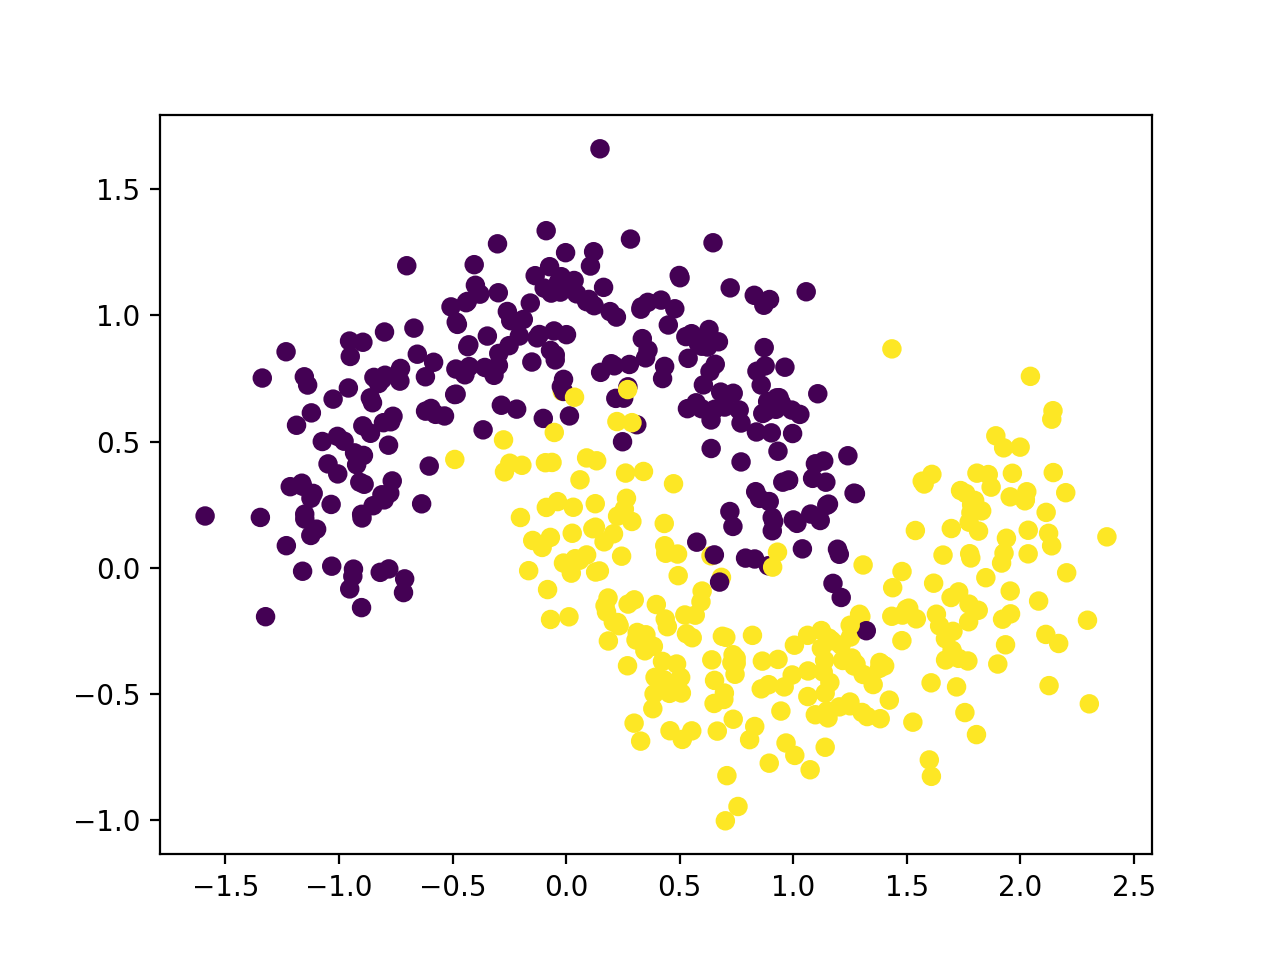
\includegraphics[width=0.8\linewidth]{moons}
      \end{figure}
\end{frame}

\begin{frame}
    \frametitle{Testing a SVM on learned features}
    % add figures
\begin{figure}[!h]
    \centering
    \begin{minipage}{.5\textwidth}
      \centering
      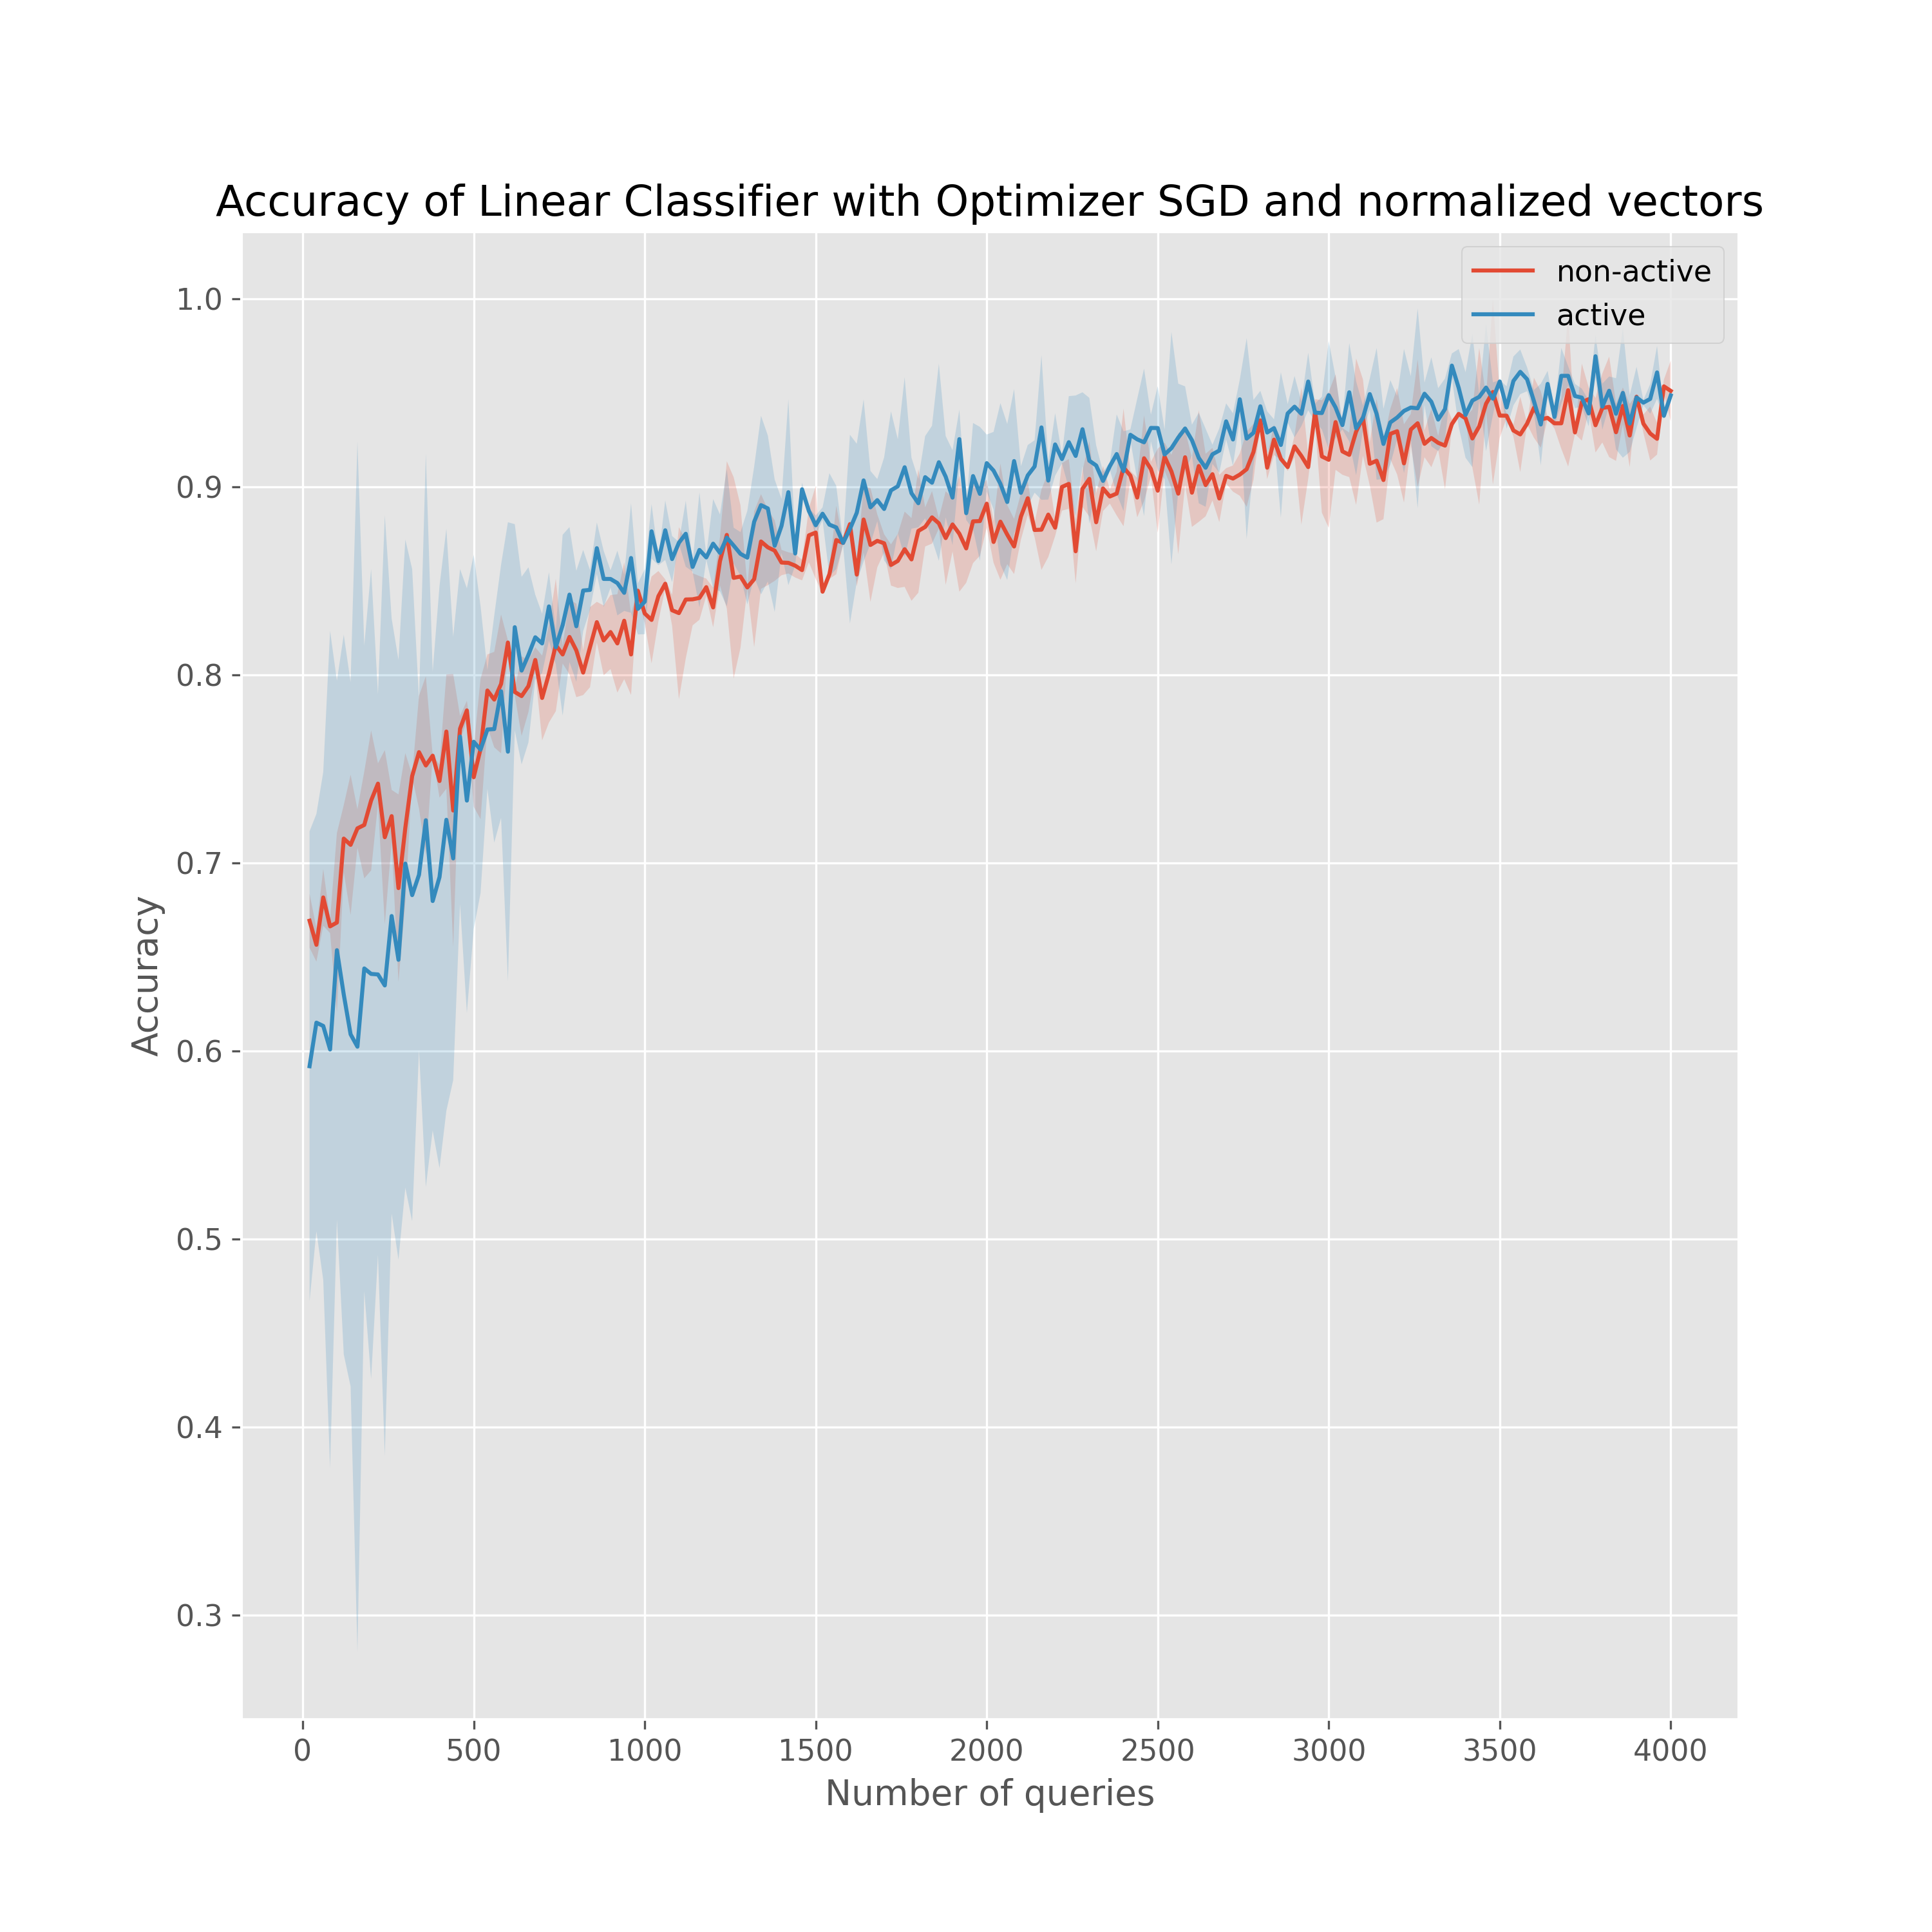
\includegraphics[width=\linewidth]{active-vs-base-moons-linear-loss-SGD-normalized-ci}
    \end{minipage}%
    \begin{minipage}{.5\textwidth}
      \centering
      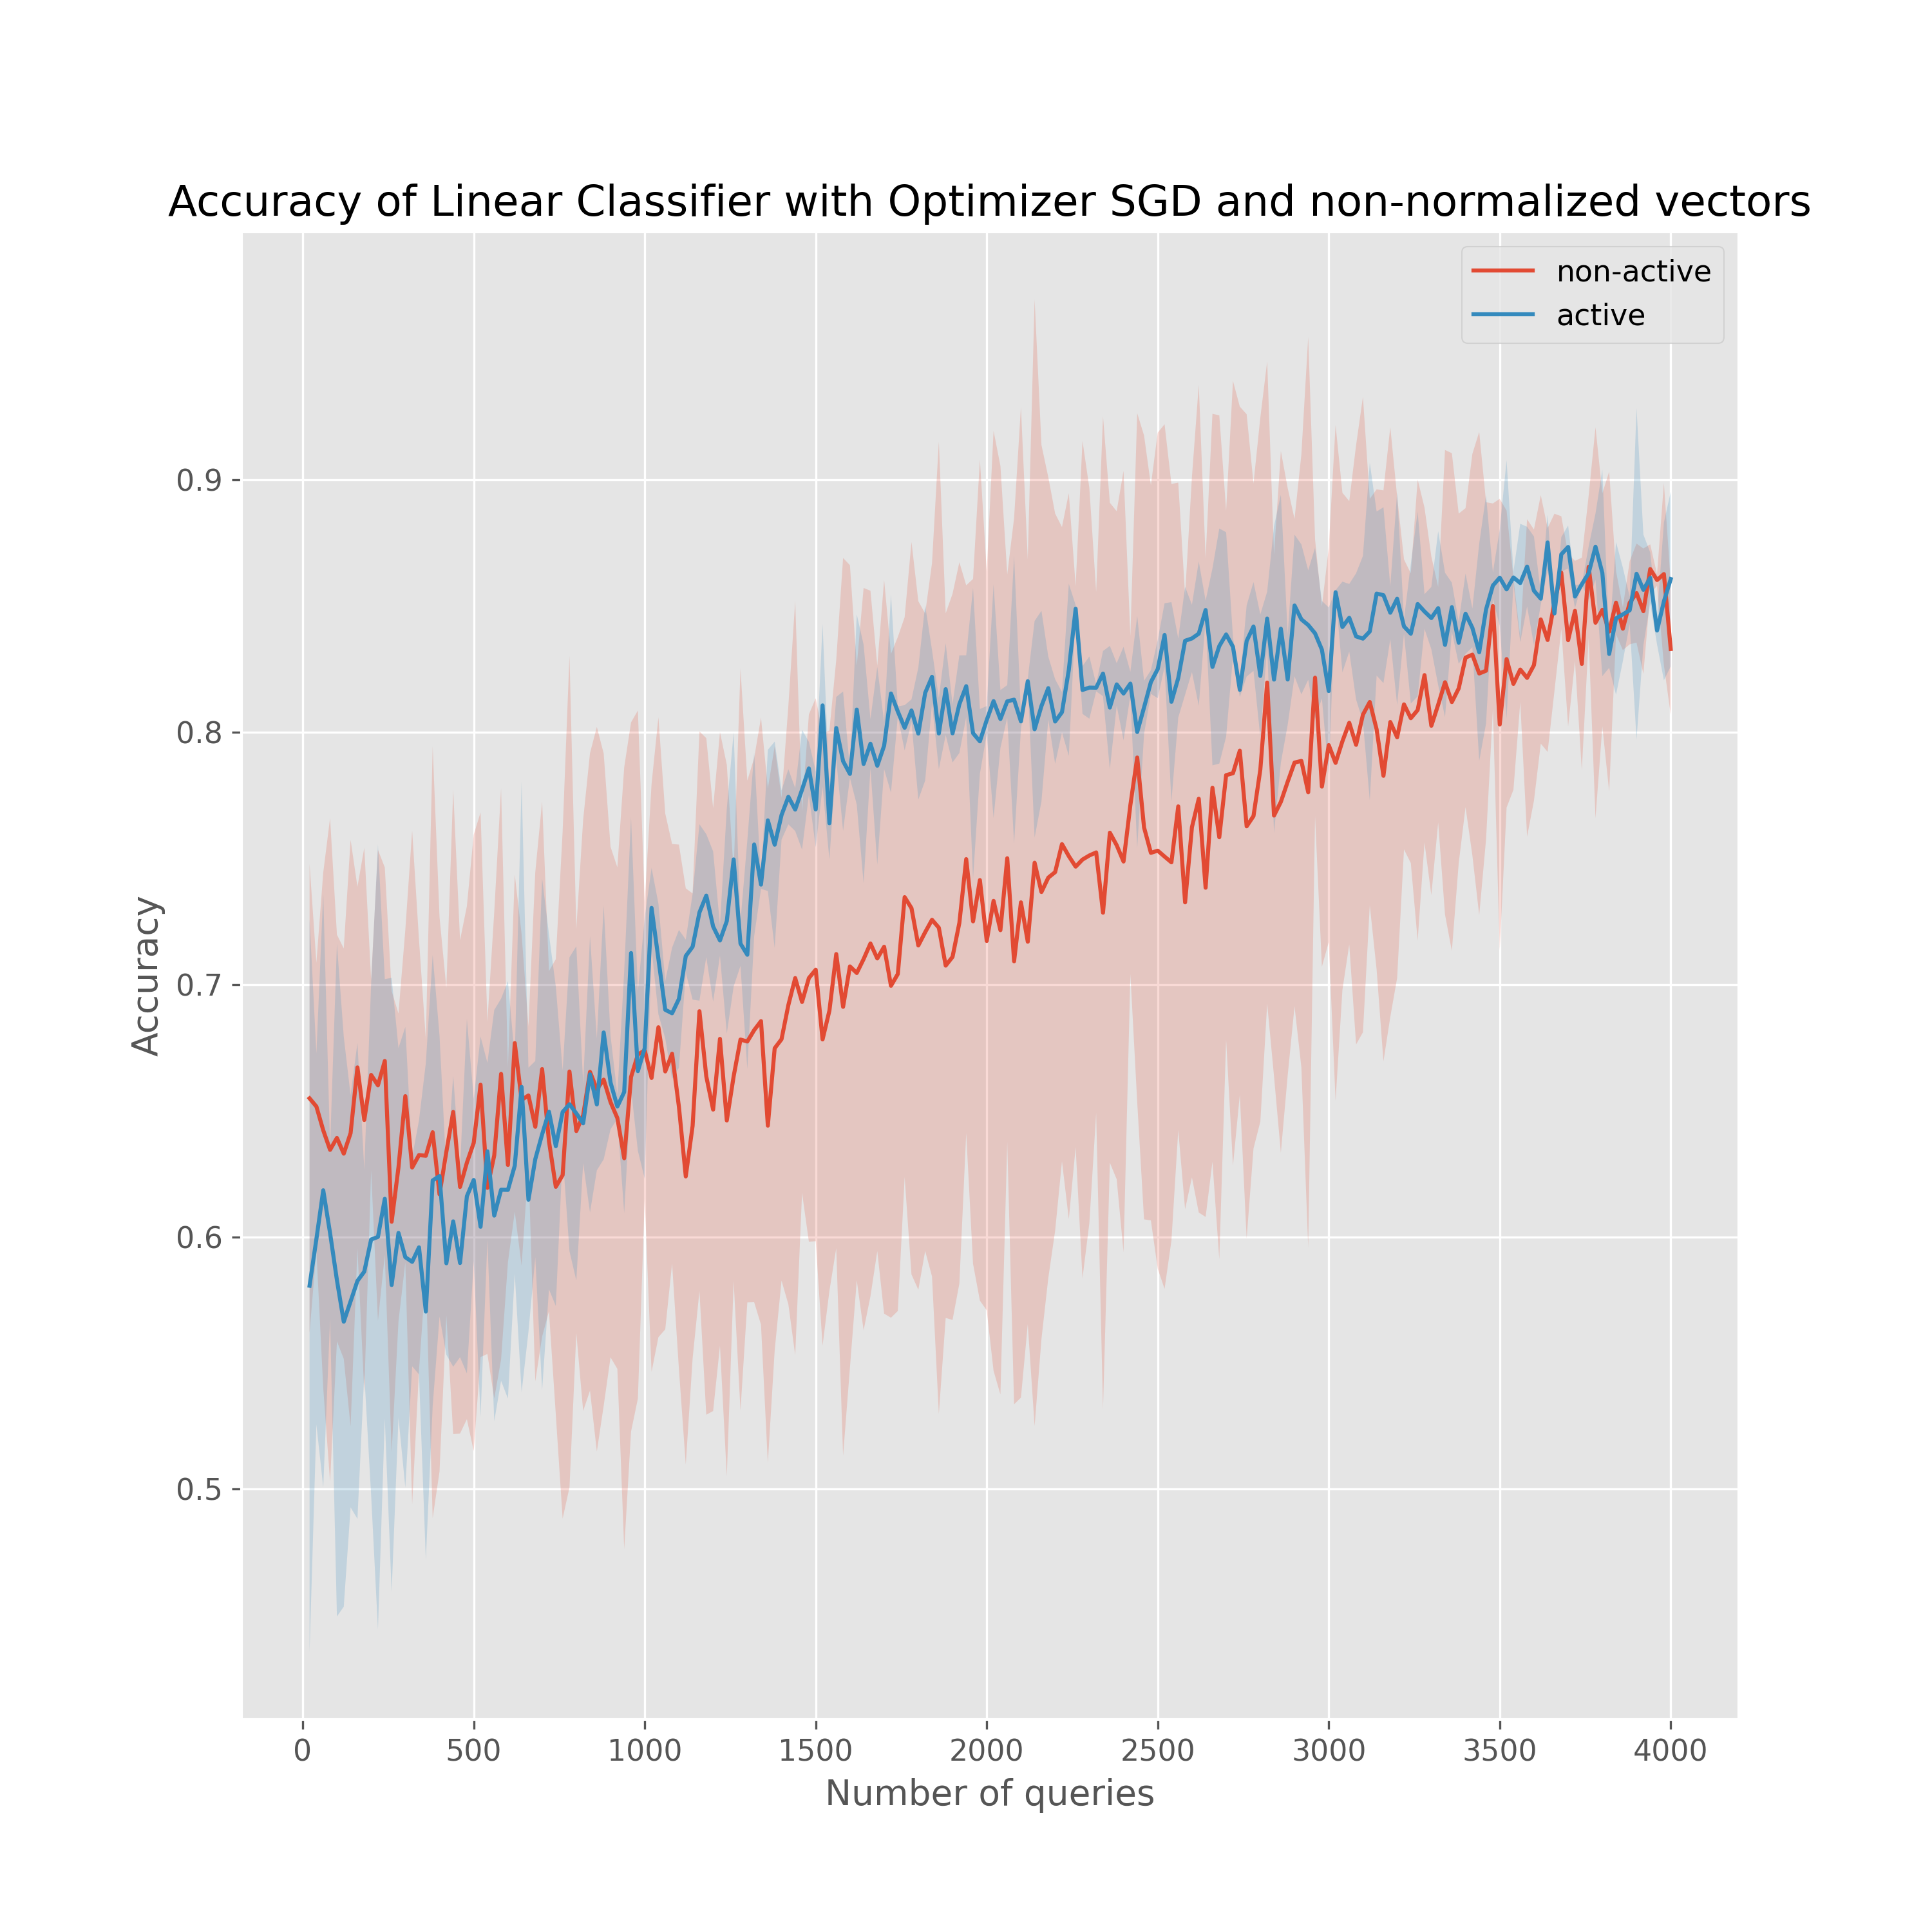
\includegraphics[width=\linewidth]{active-vs-base-moons-linear-loss-SGD-non-normalized-ci}
    \end{minipage}
    \caption{Performance SVM}
  \end{figure}
\end{frame}

\begin{frame}{}
    \frametitle{Comparing L2 loss of learned features}
    % add figures
\begin{figure}[!h]
    \centering
    \begin{minipage}{.5\textwidth}
      \centering
      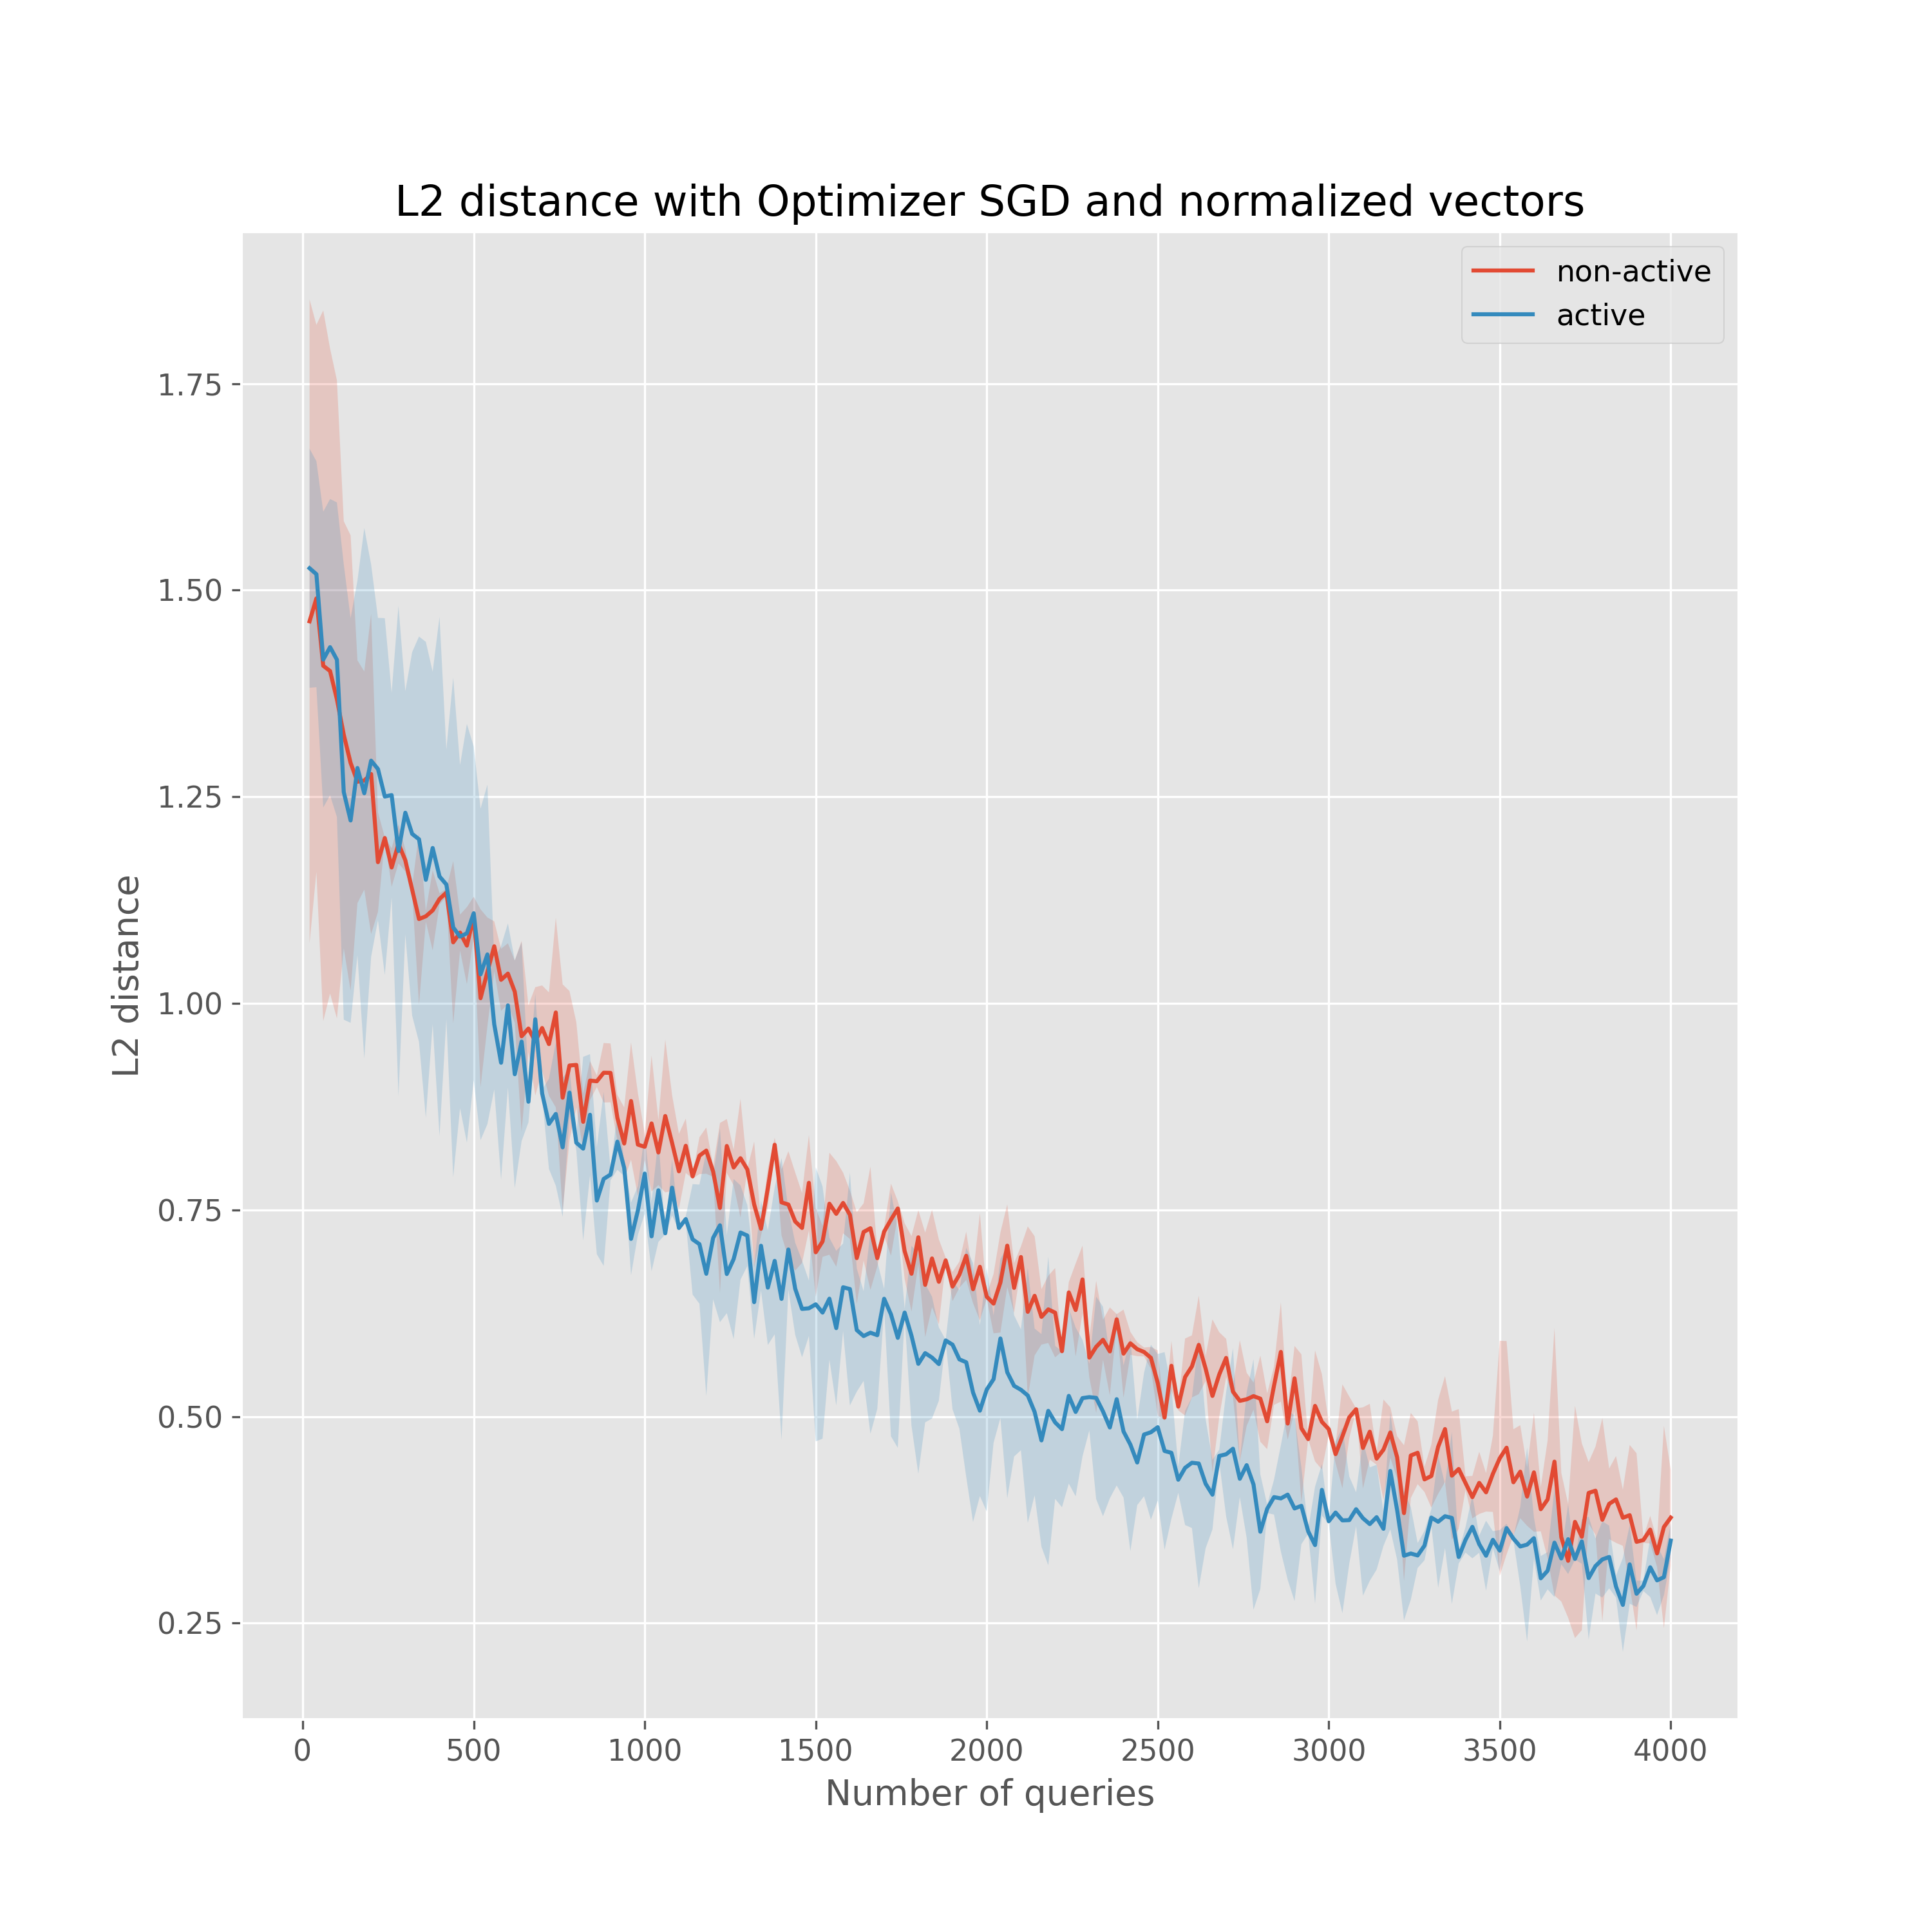
\includegraphics[width=\linewidth]{active-vs-base-moons-l2-loss-SGD-normalized-ci}
    \end{minipage}%
    \begin{minipage}{.5\textwidth}
      \centering
      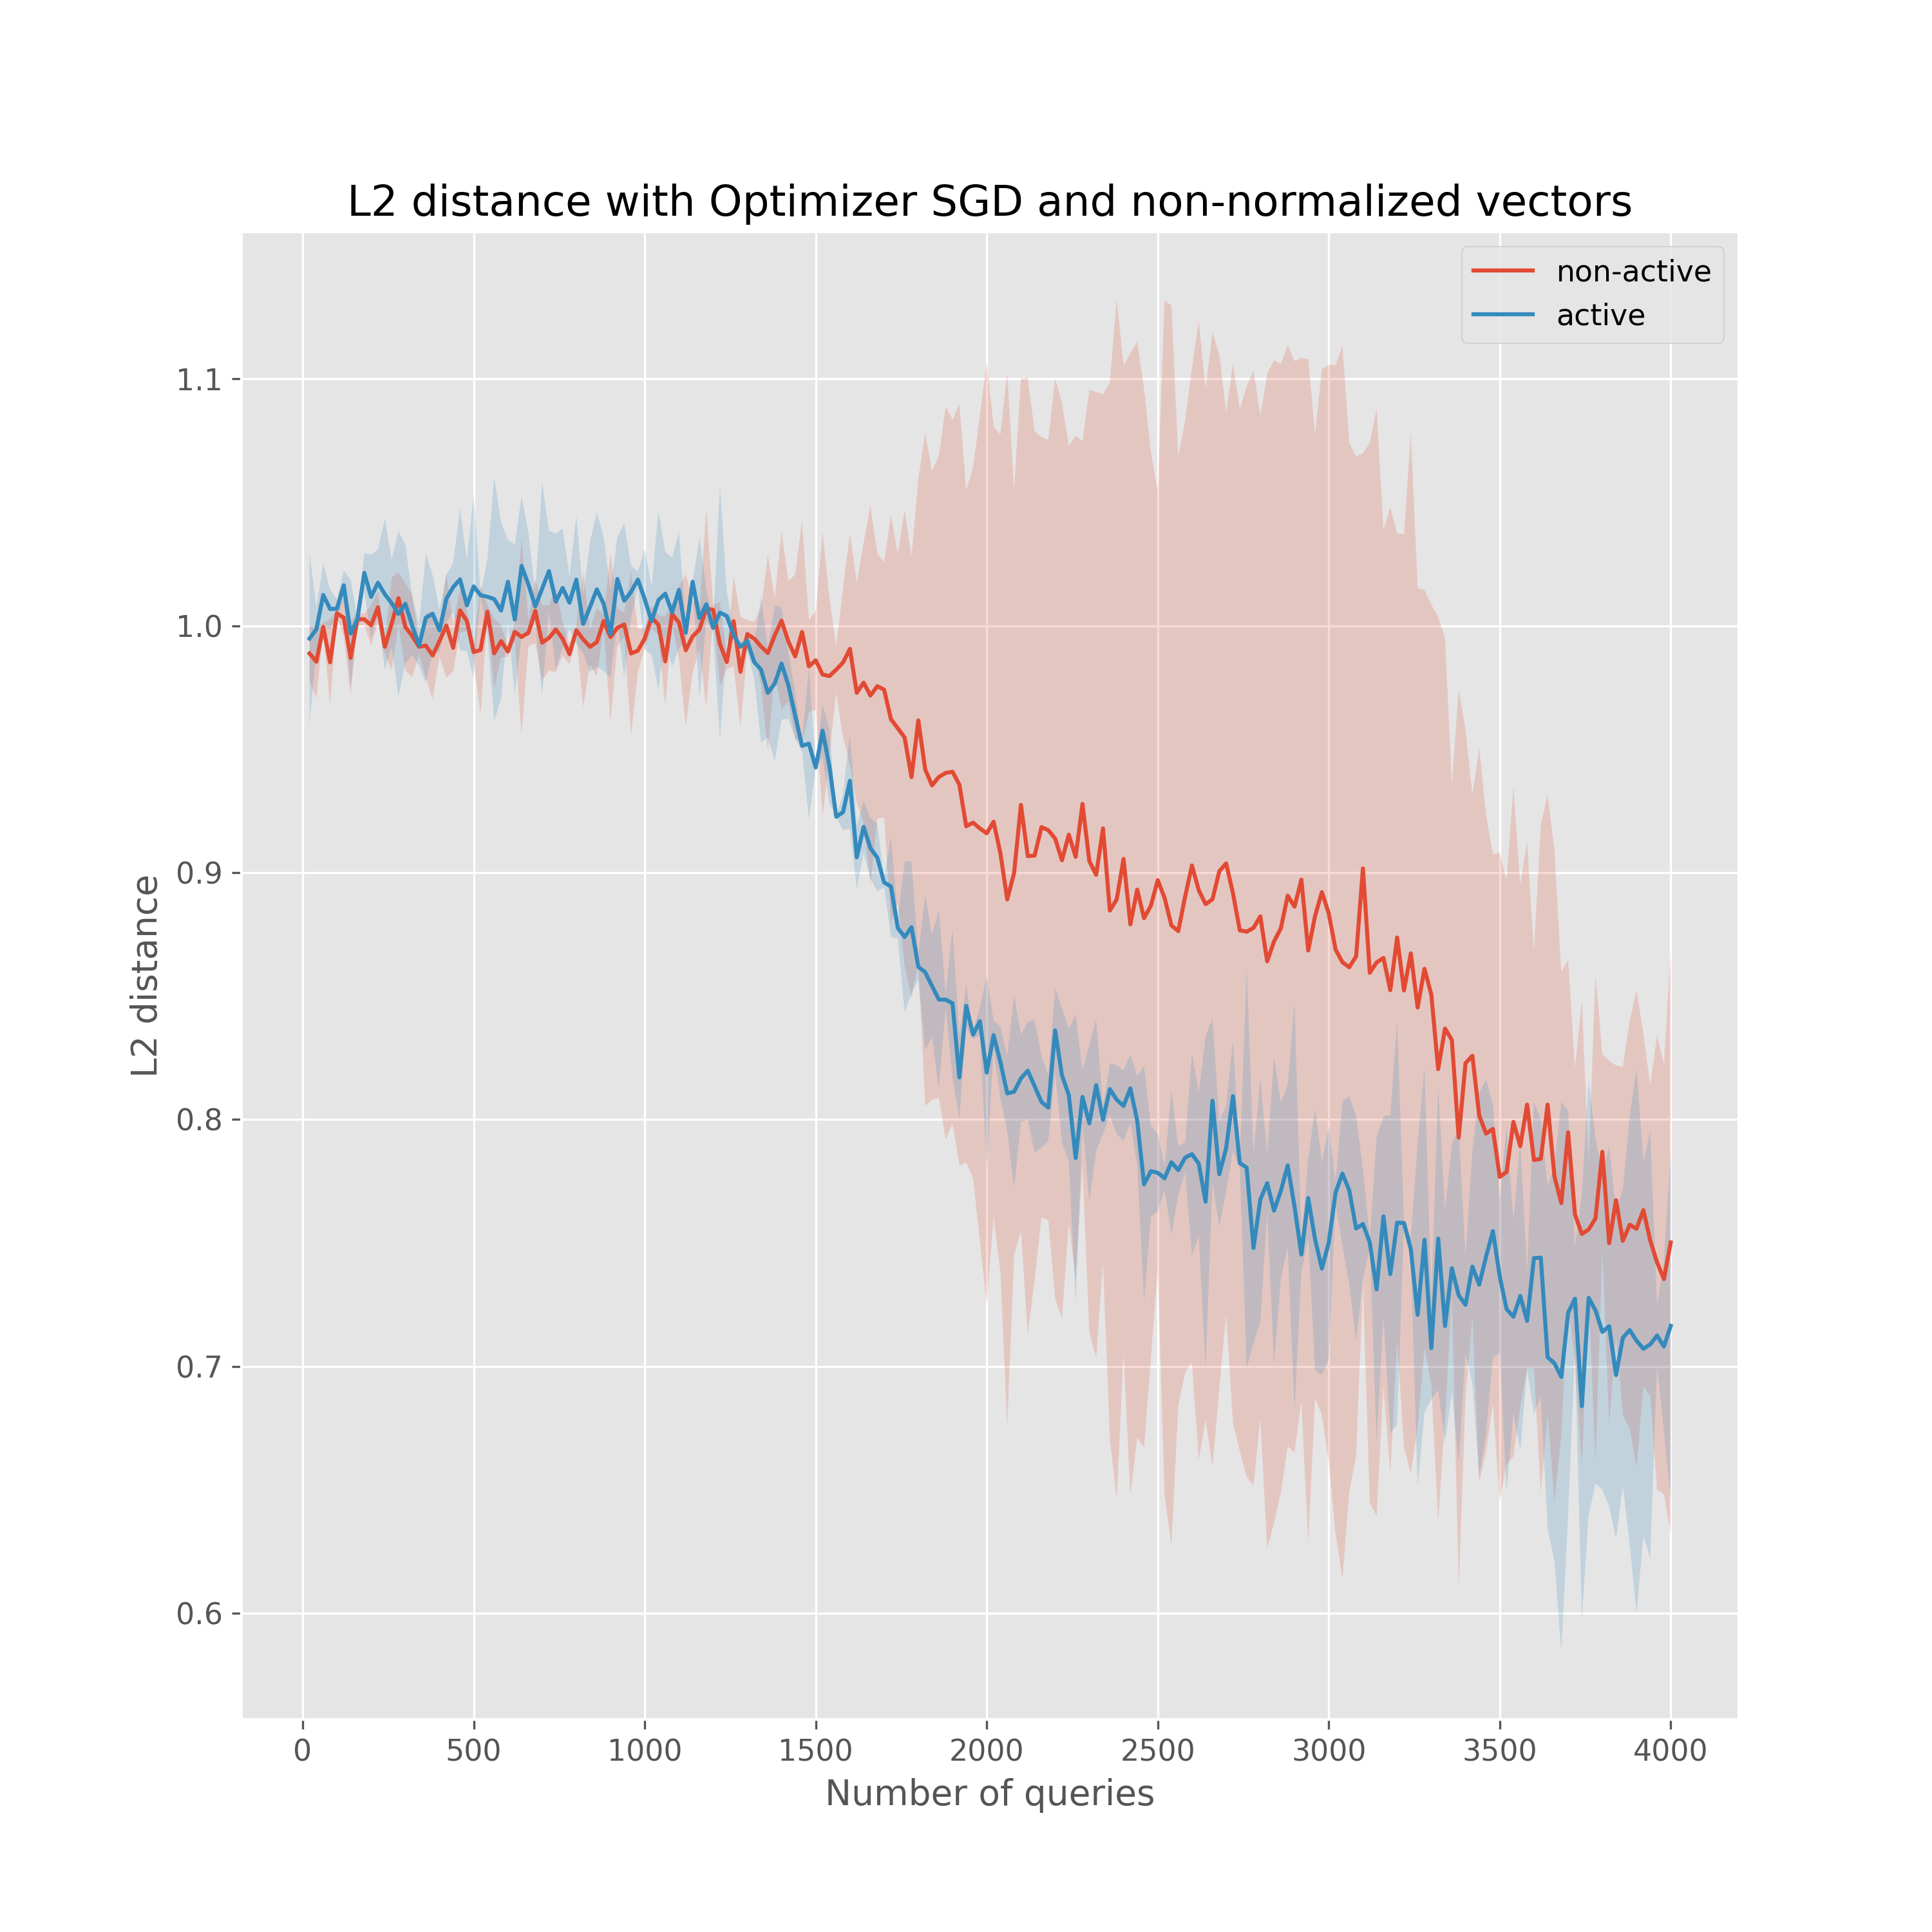
\includegraphics[width=\linewidth]{active-vs-base-moons-l2-loss-SGD-non-normalized-ci}
    \end{minipage}
    \caption{Performance SVM}
  \end{figure}
\end{frame}

\begin{frame}
    \frametitle{Empirical test on blobs:}
    % add figures
\begin{figure}[!h]
    \centering
    \begin{minipage}{.5\textwidth}
      \centering
      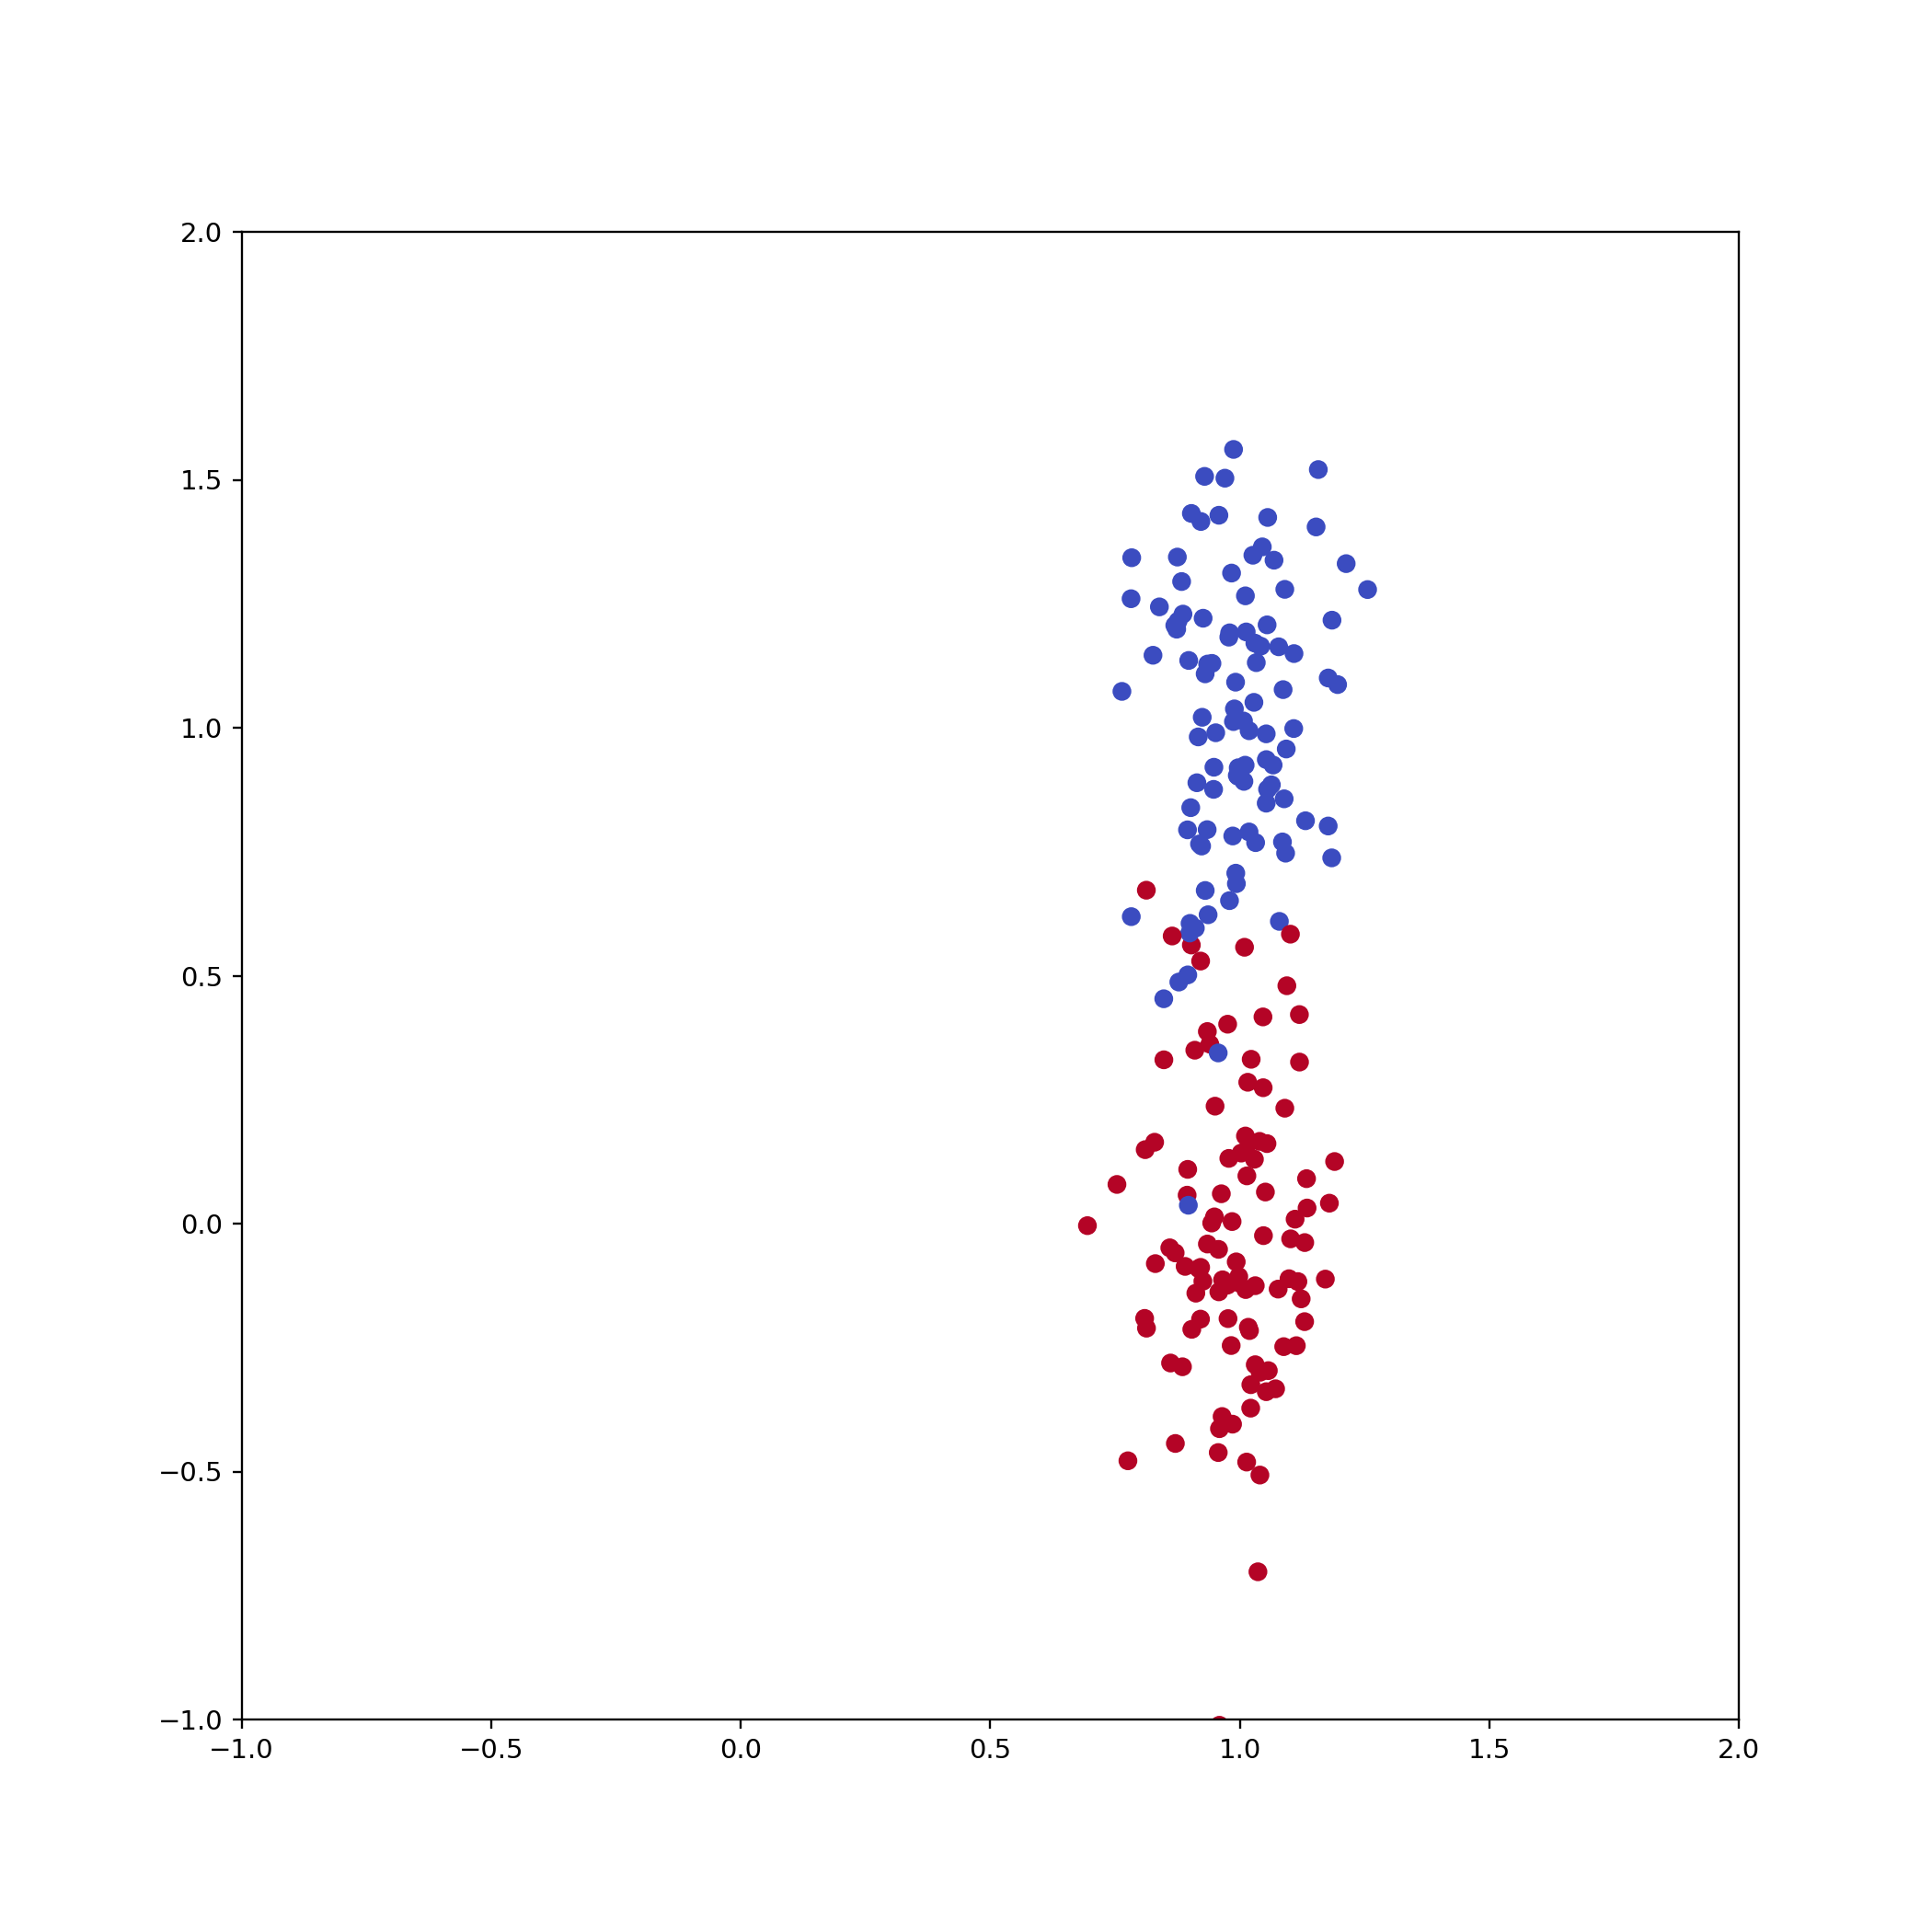
\includegraphics[width=\linewidth]{blobs-balanced}
    \end{minipage}%
    \begin{minipage}{.5\textwidth}
      \centering
      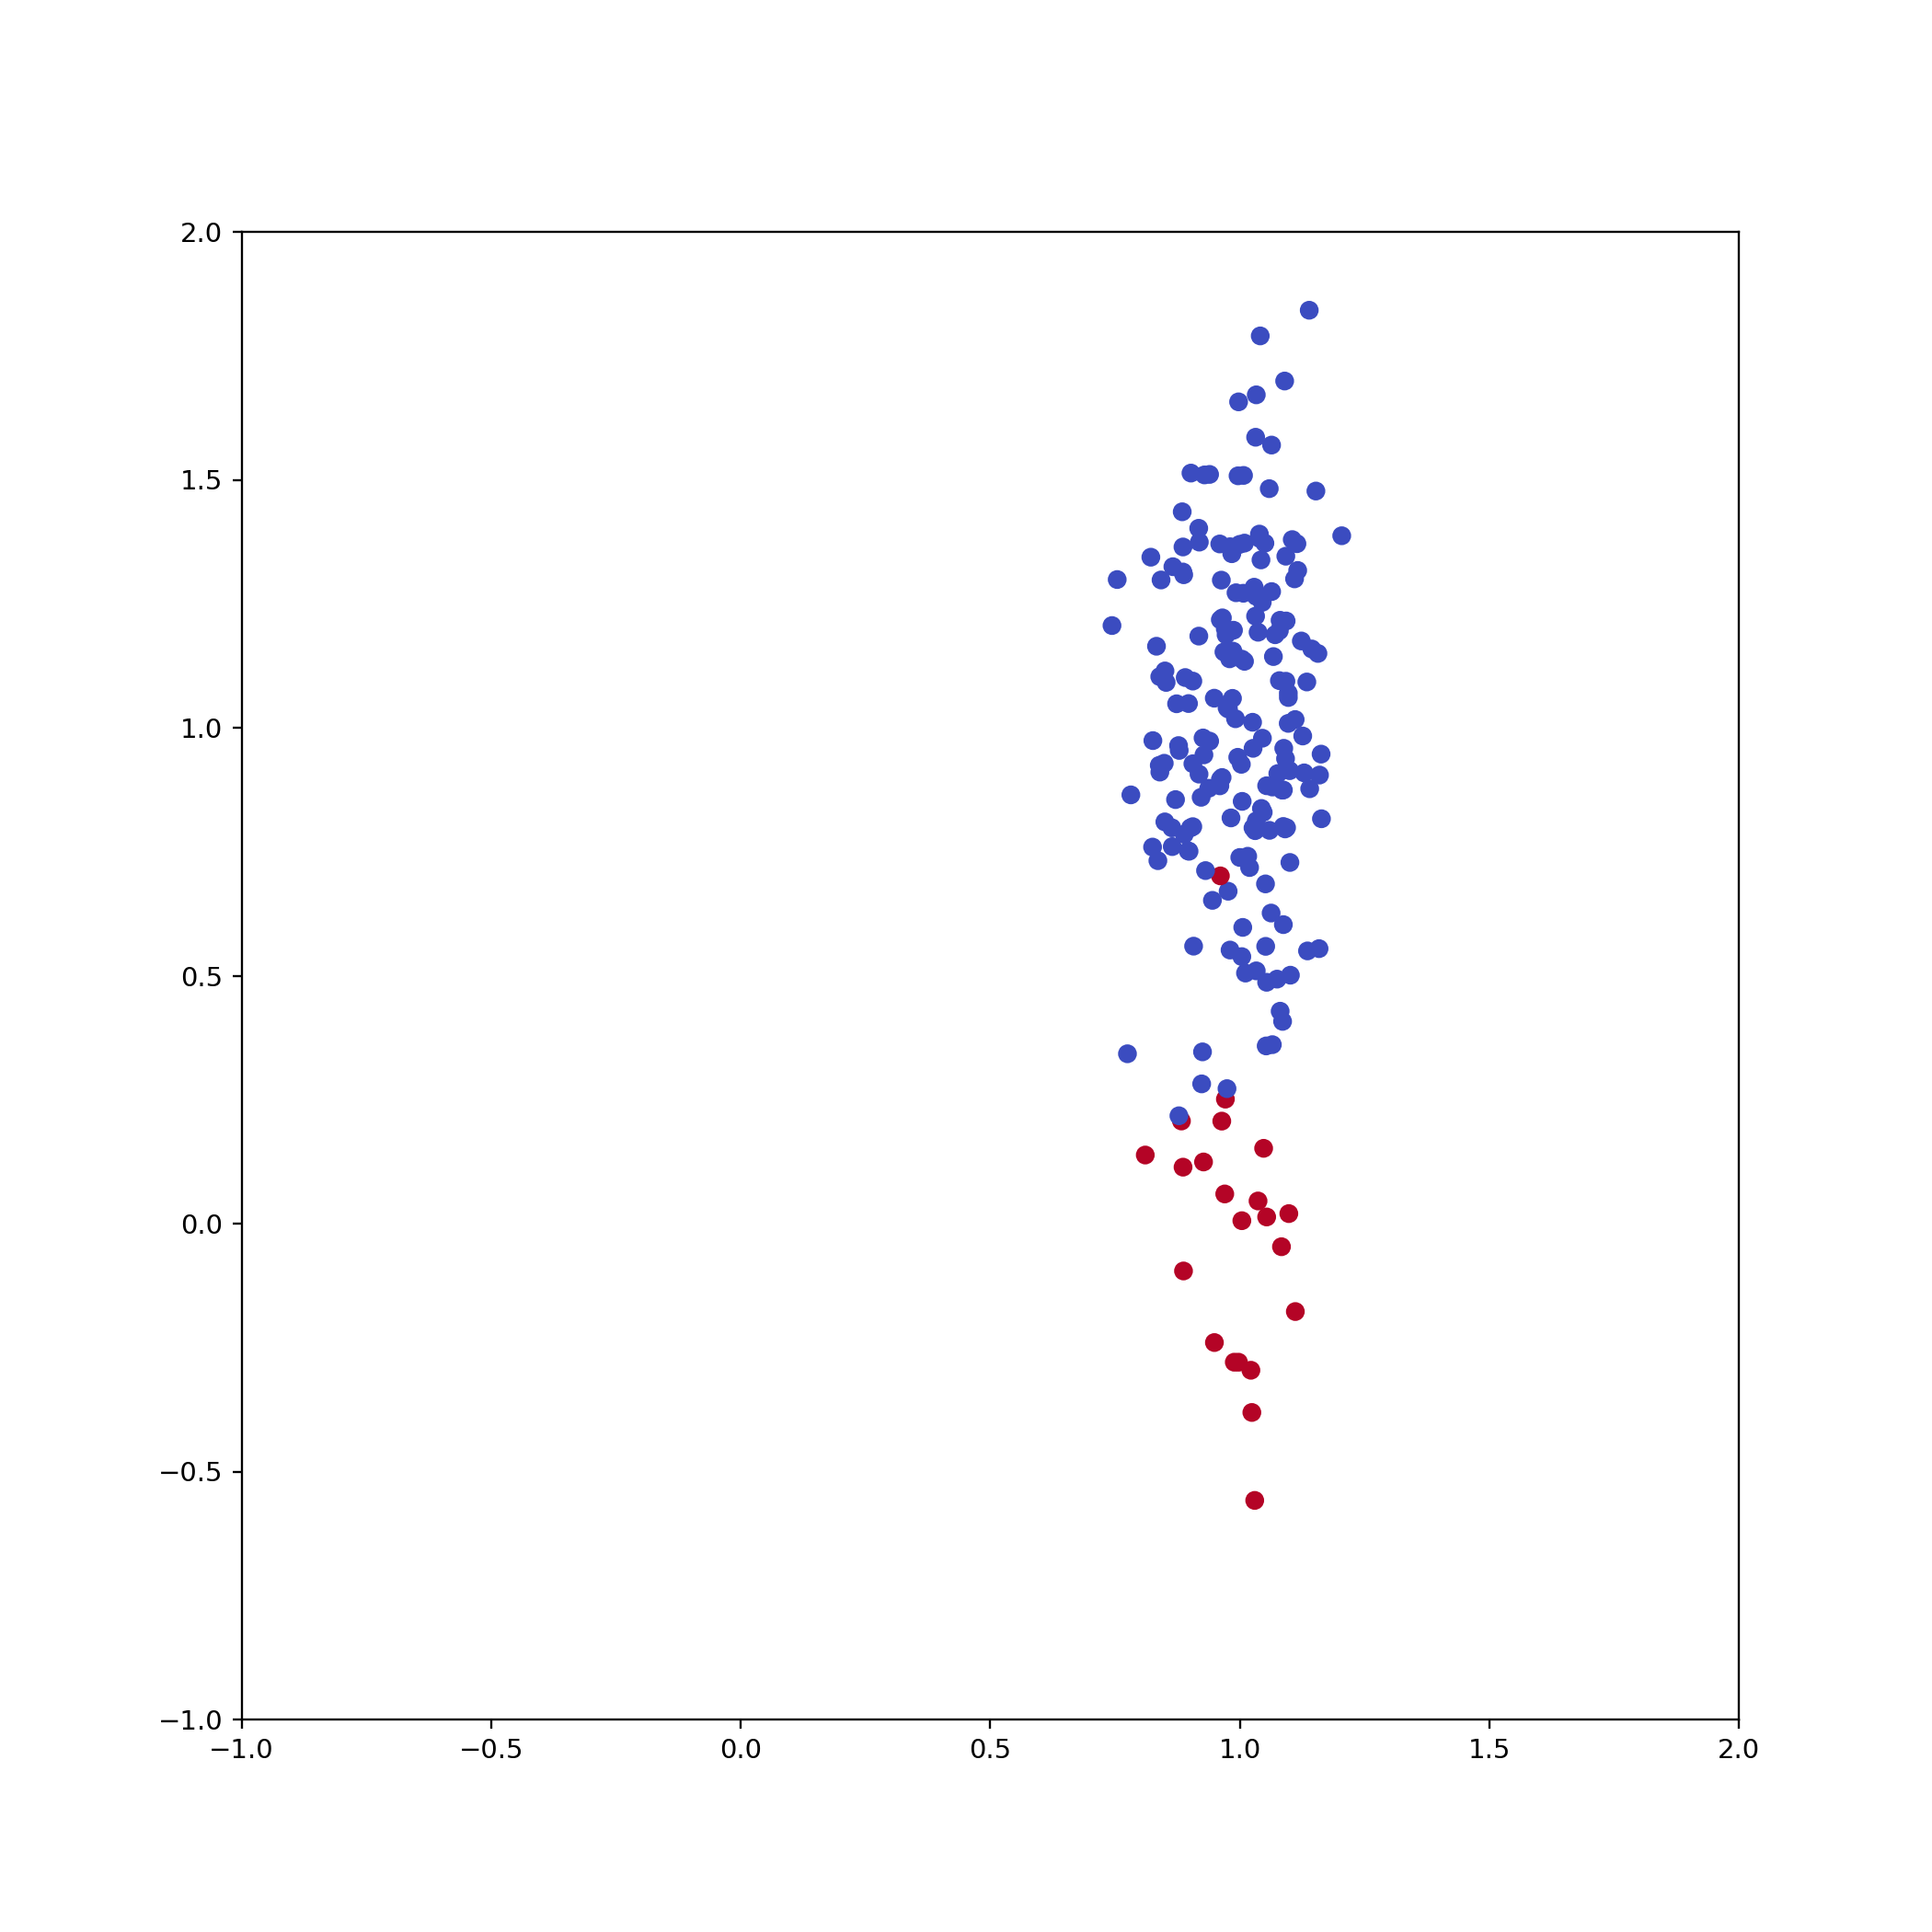
\includegraphics[width=\linewidth]{blobs-unbalanced}
    \end{minipage}
    \caption{Performance SVM}
  \end{figure}
\end{frame}




\begin{frame}{}
    \frametitle{Results}
    \begin{figure}[!h]
      \centering
      \begin{minipage}{.45\textwidth}
        \centering
        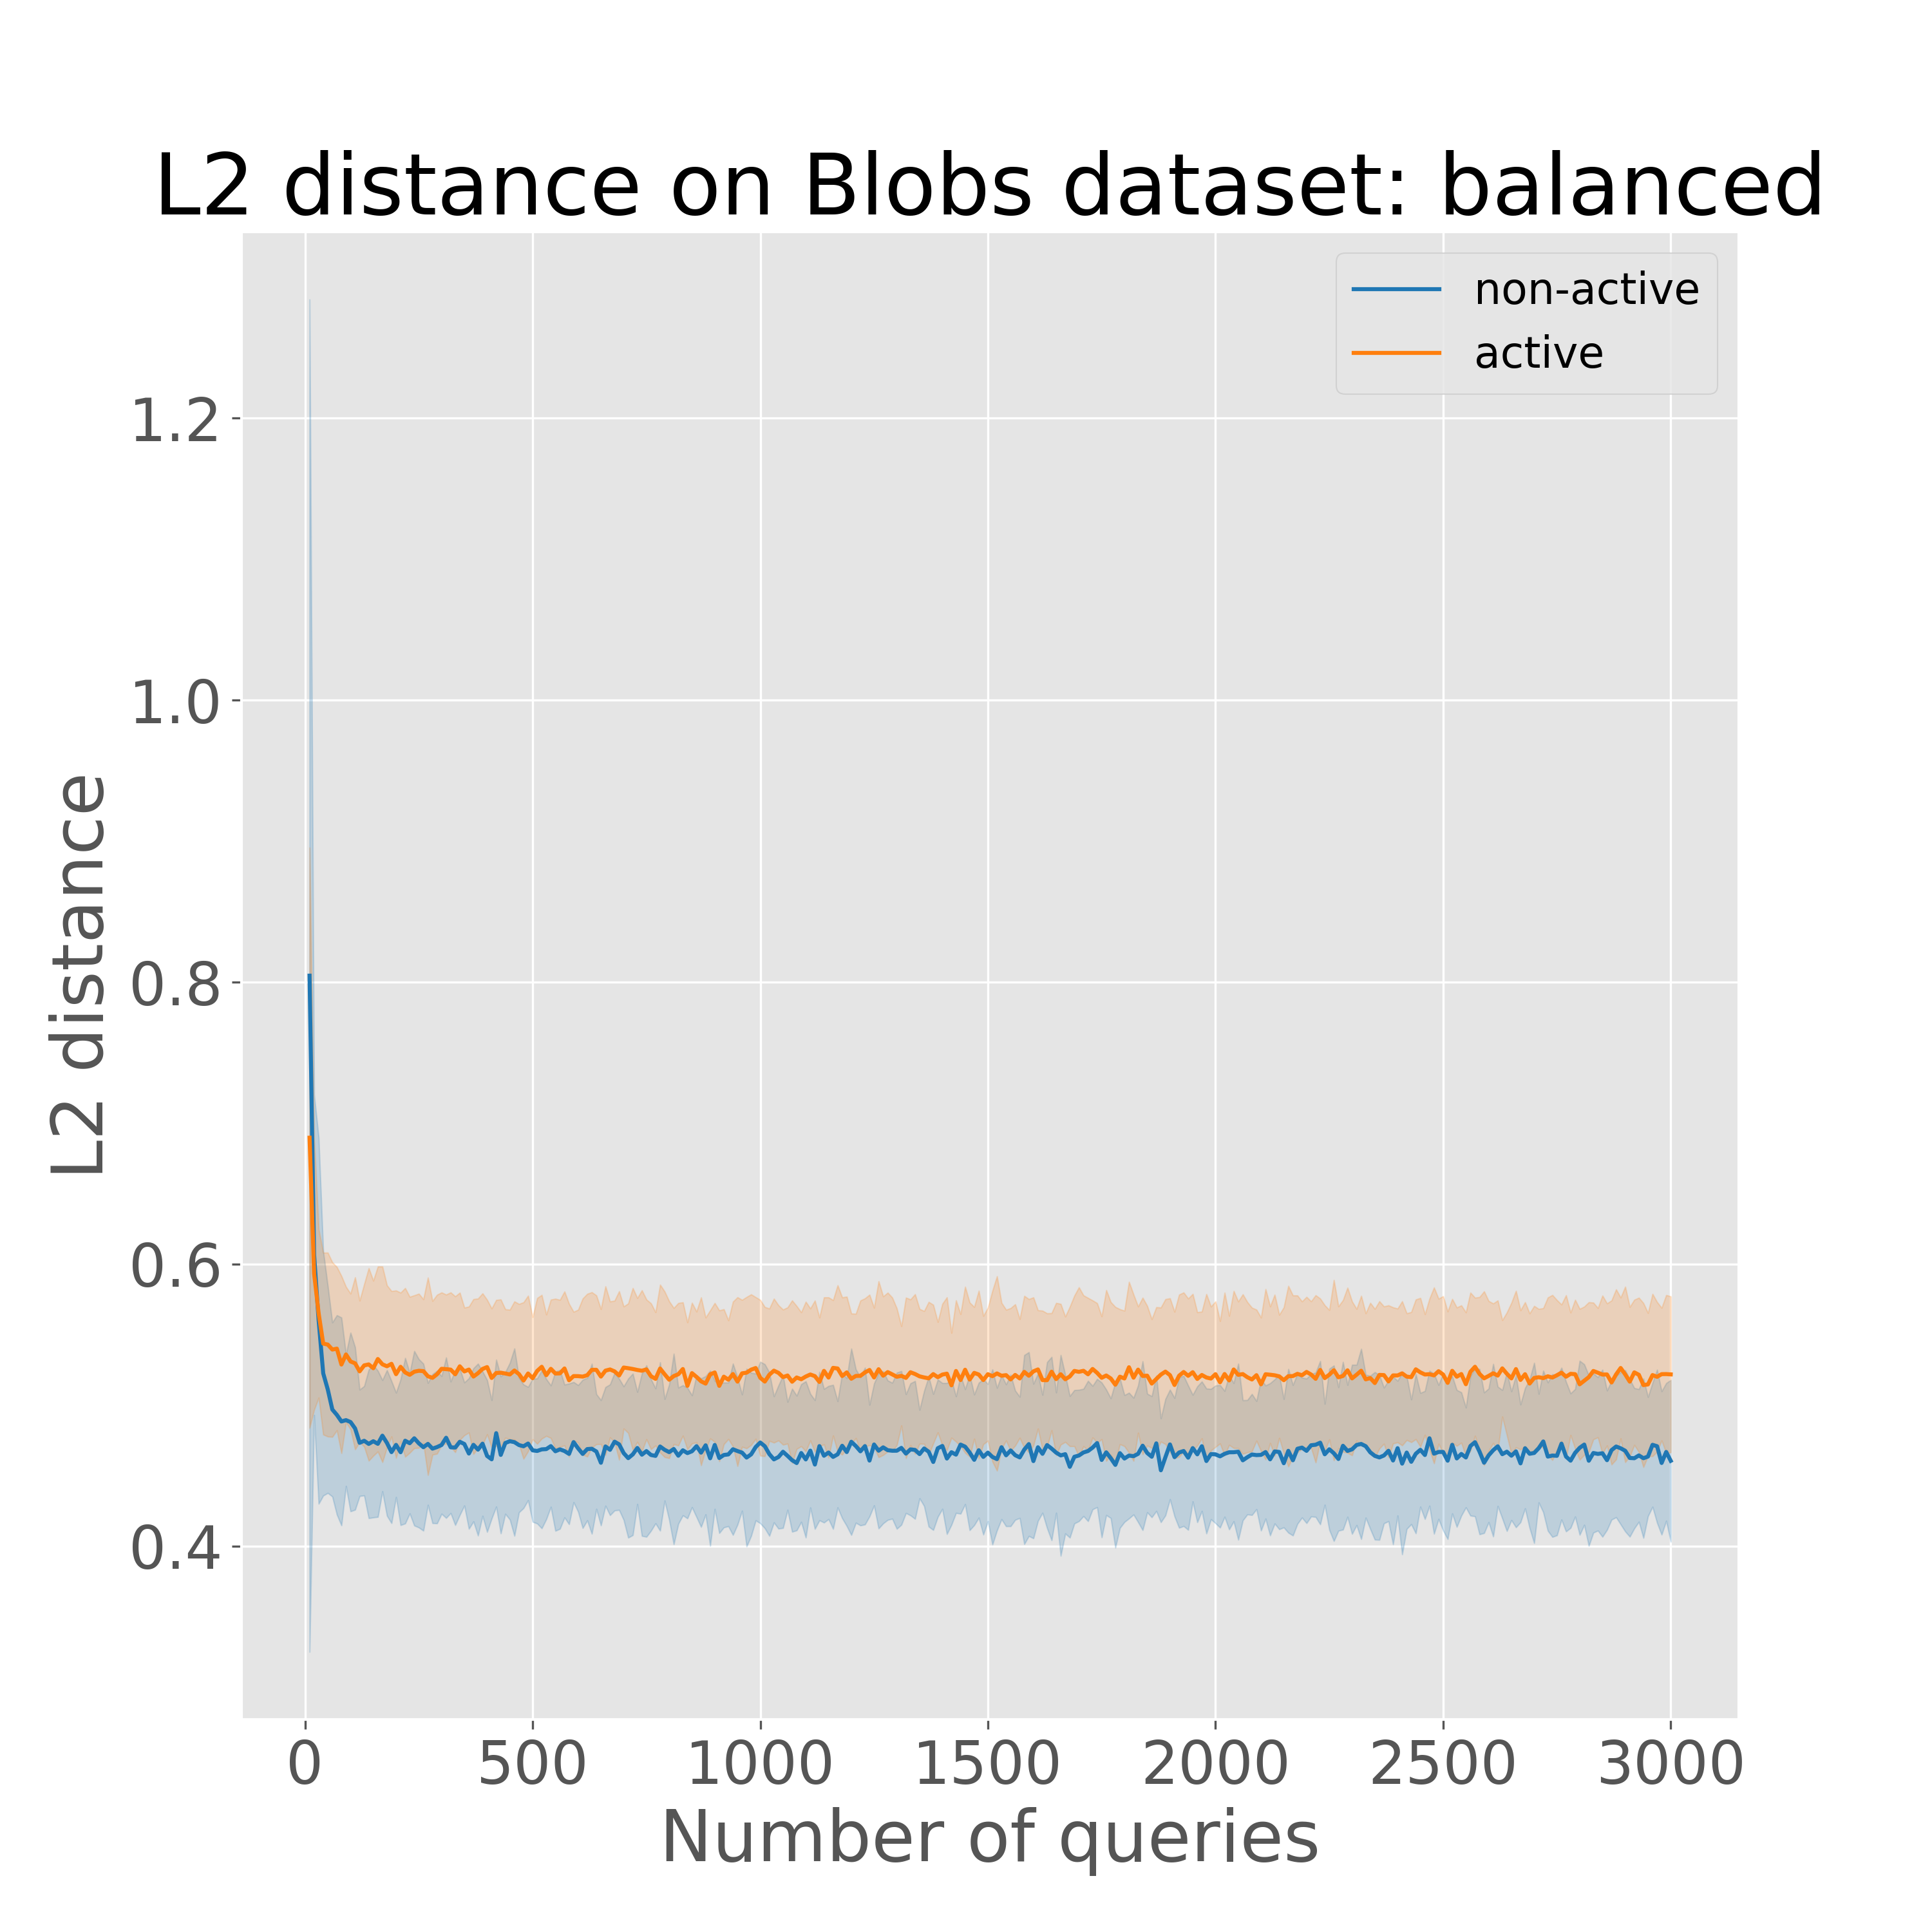
\includegraphics[width=\linewidth]{active-vs-base-blobs-l2-loss_balanced-ci}
        \caption{Balanced dataset}\label{fig:linucb-blobs-l2-loss-balanced}
      \end{minipage}%
      \begin{minipage}{.45\textwidth}
        \centering
        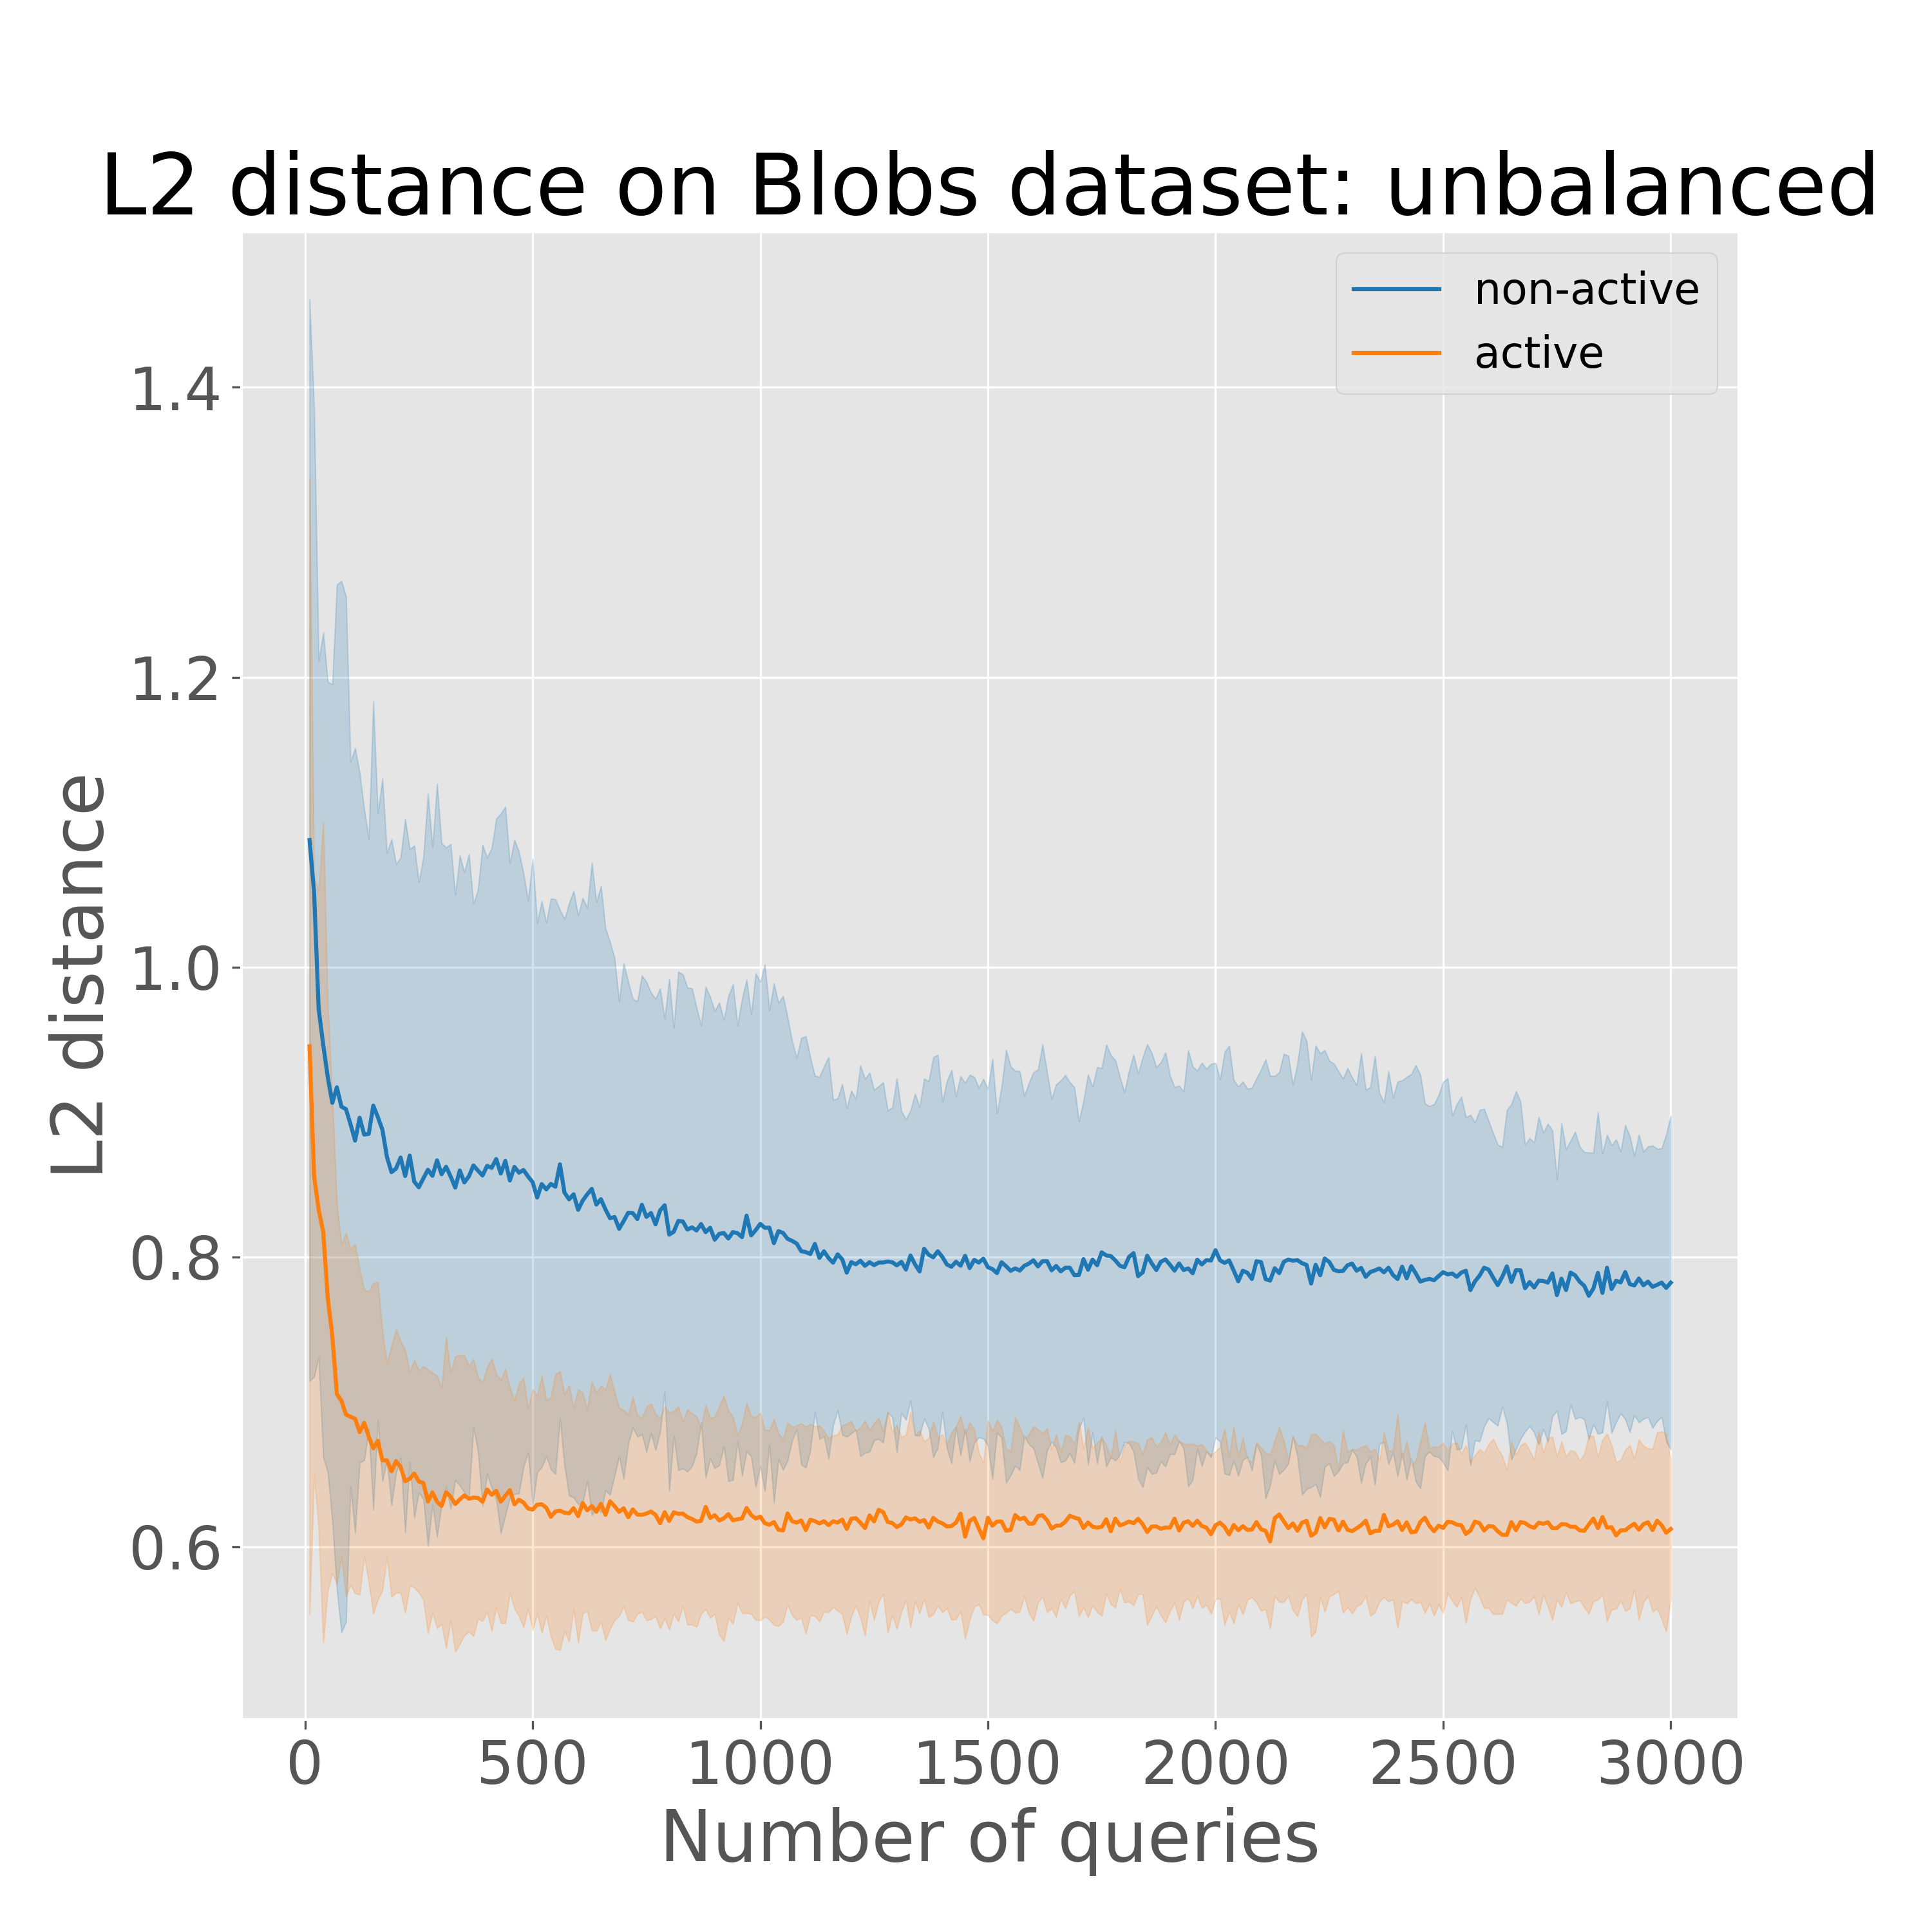
\includegraphics[width=\linewidth]{active-vs-base-blobs-l2-loss_unbalanced-ci}
        \caption{Unbalanced dataset}\label{fig:linucb-blobs-l2-loss-unbalanced}
      \end{minipage}
    \end{figure}
\end{frame}


\begin{frame}{}
    \frametitle{Results}

\begin{figure}[!h]
  \centering
  \begin{minipage}{.45\textwidth}
    \centering
    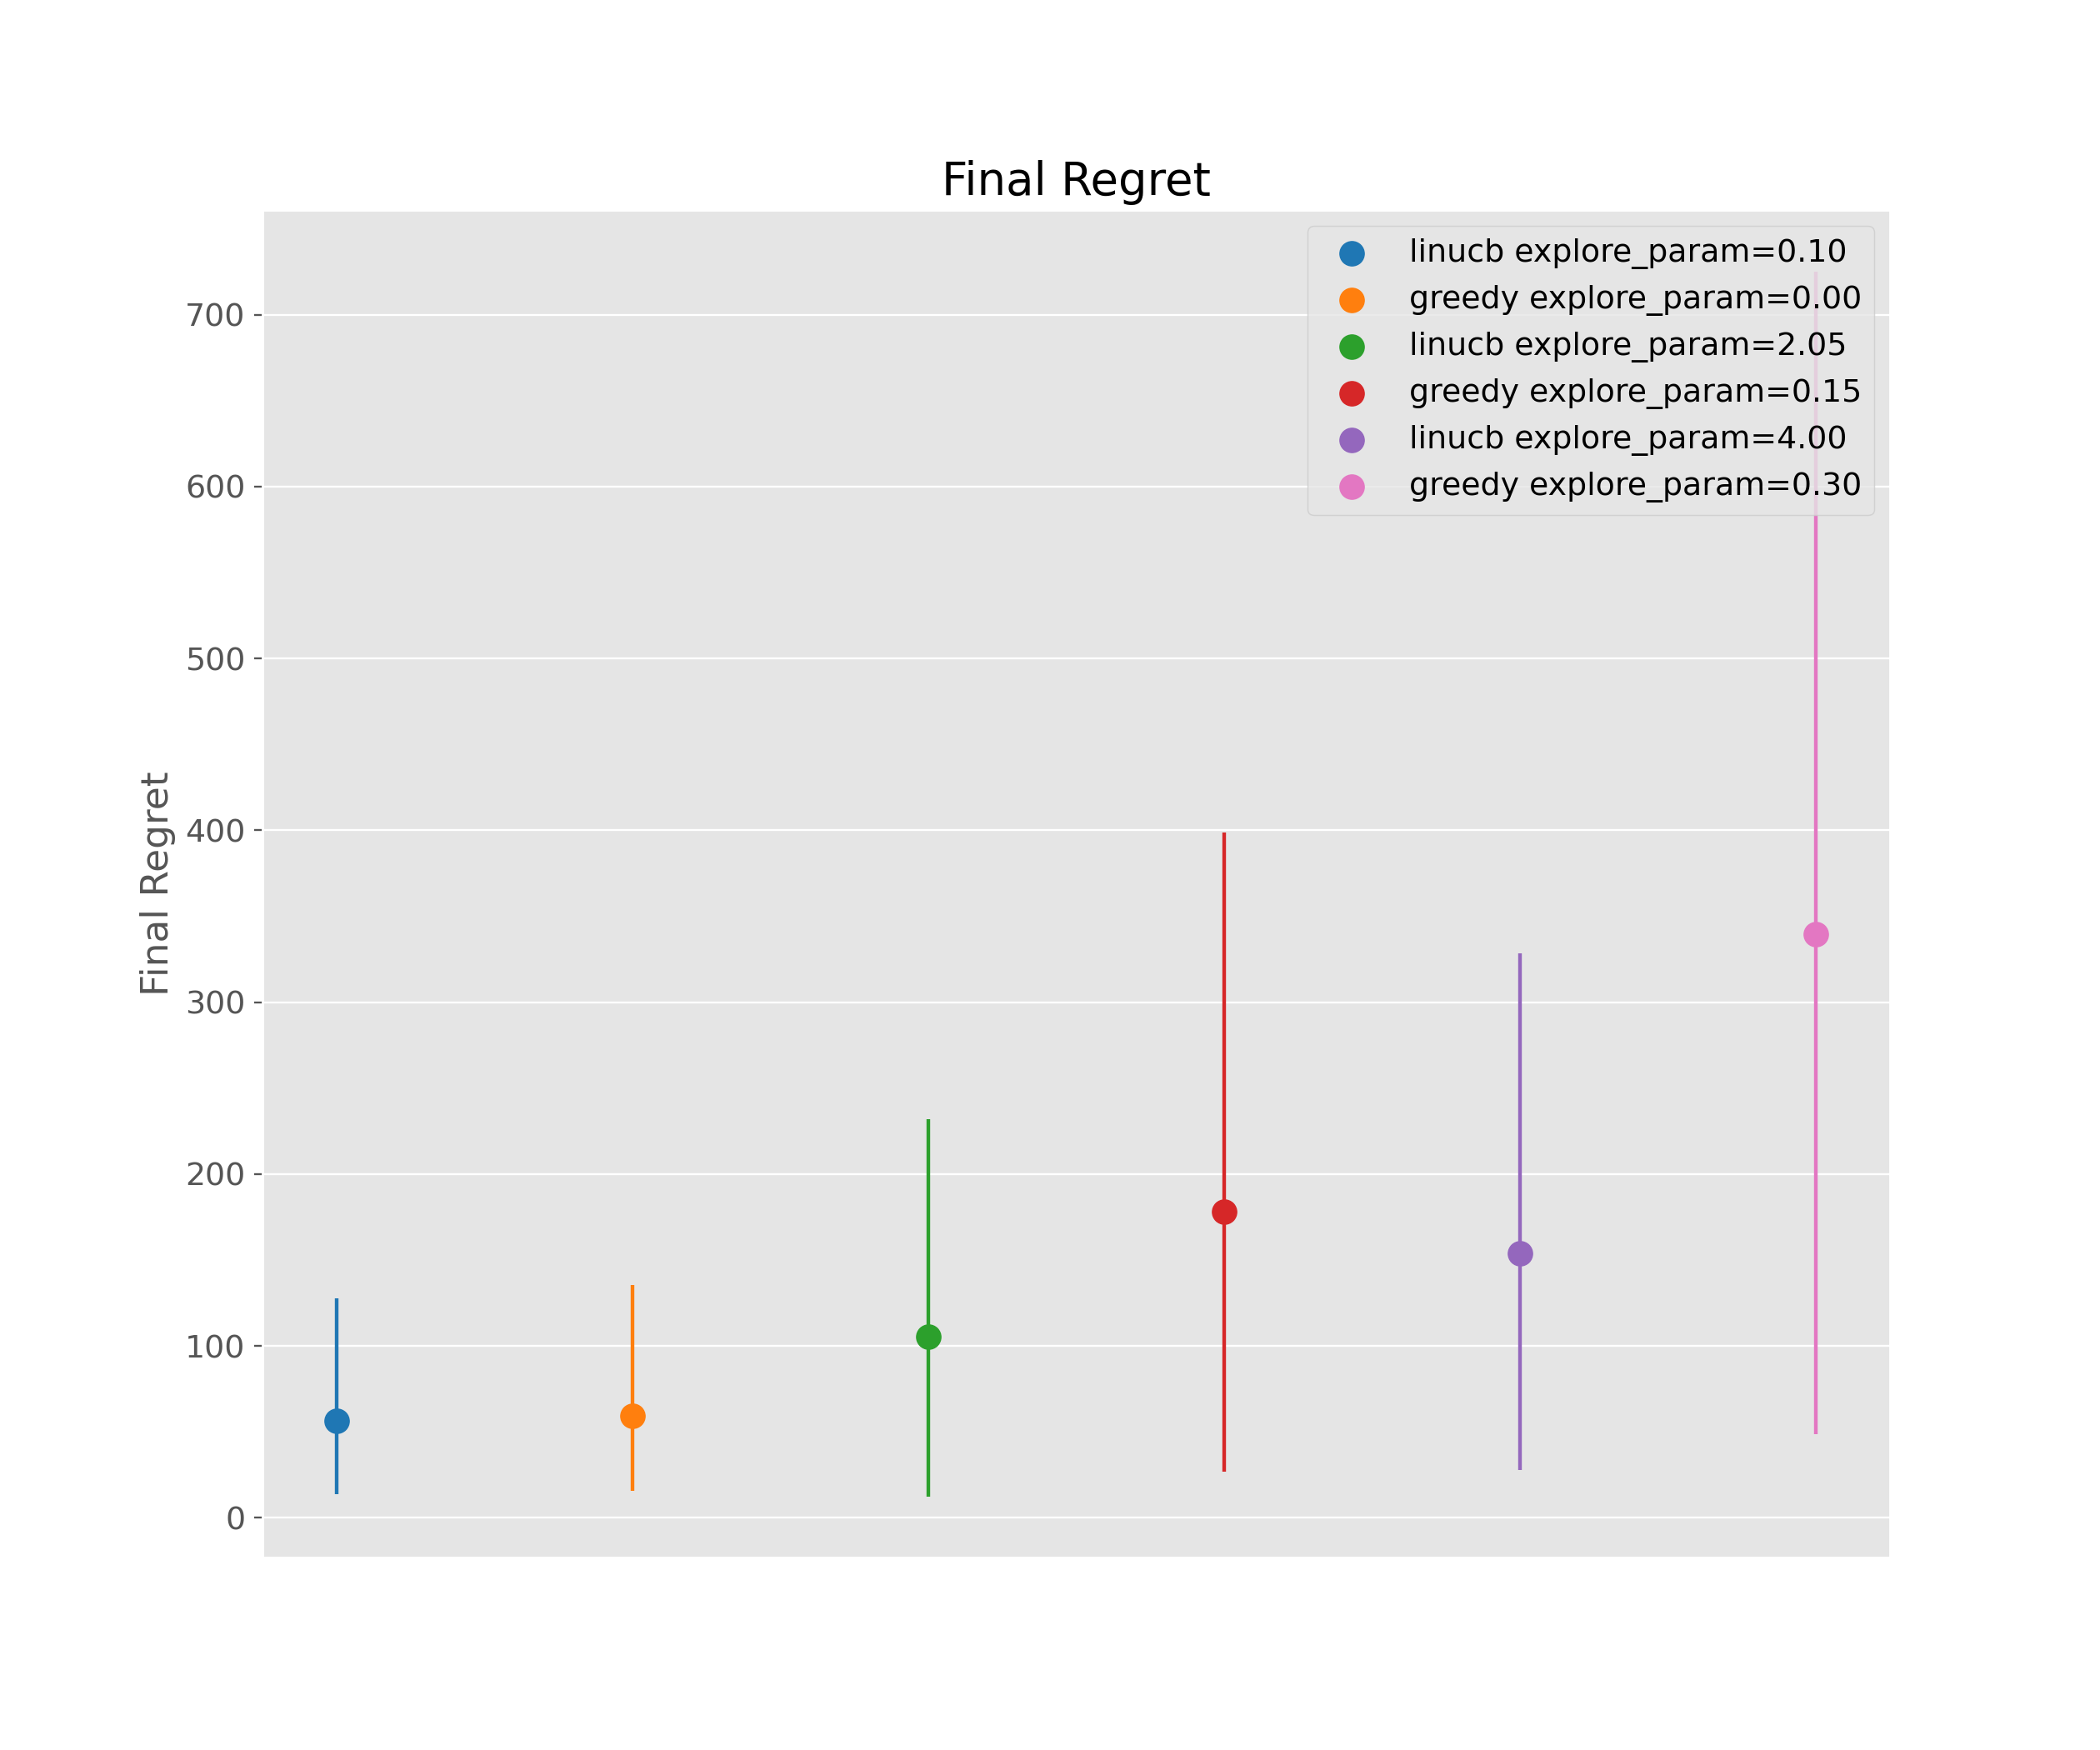
\includegraphics[width=\linewidth]{epsilon_vs_linucb_blobs}
    \caption{Regret without regime change}\label{fig:linucb-blobs-regret-no-regime-change}
  \end{minipage}%
  \begin{minipage}{.45\textwidth}
    \centering
    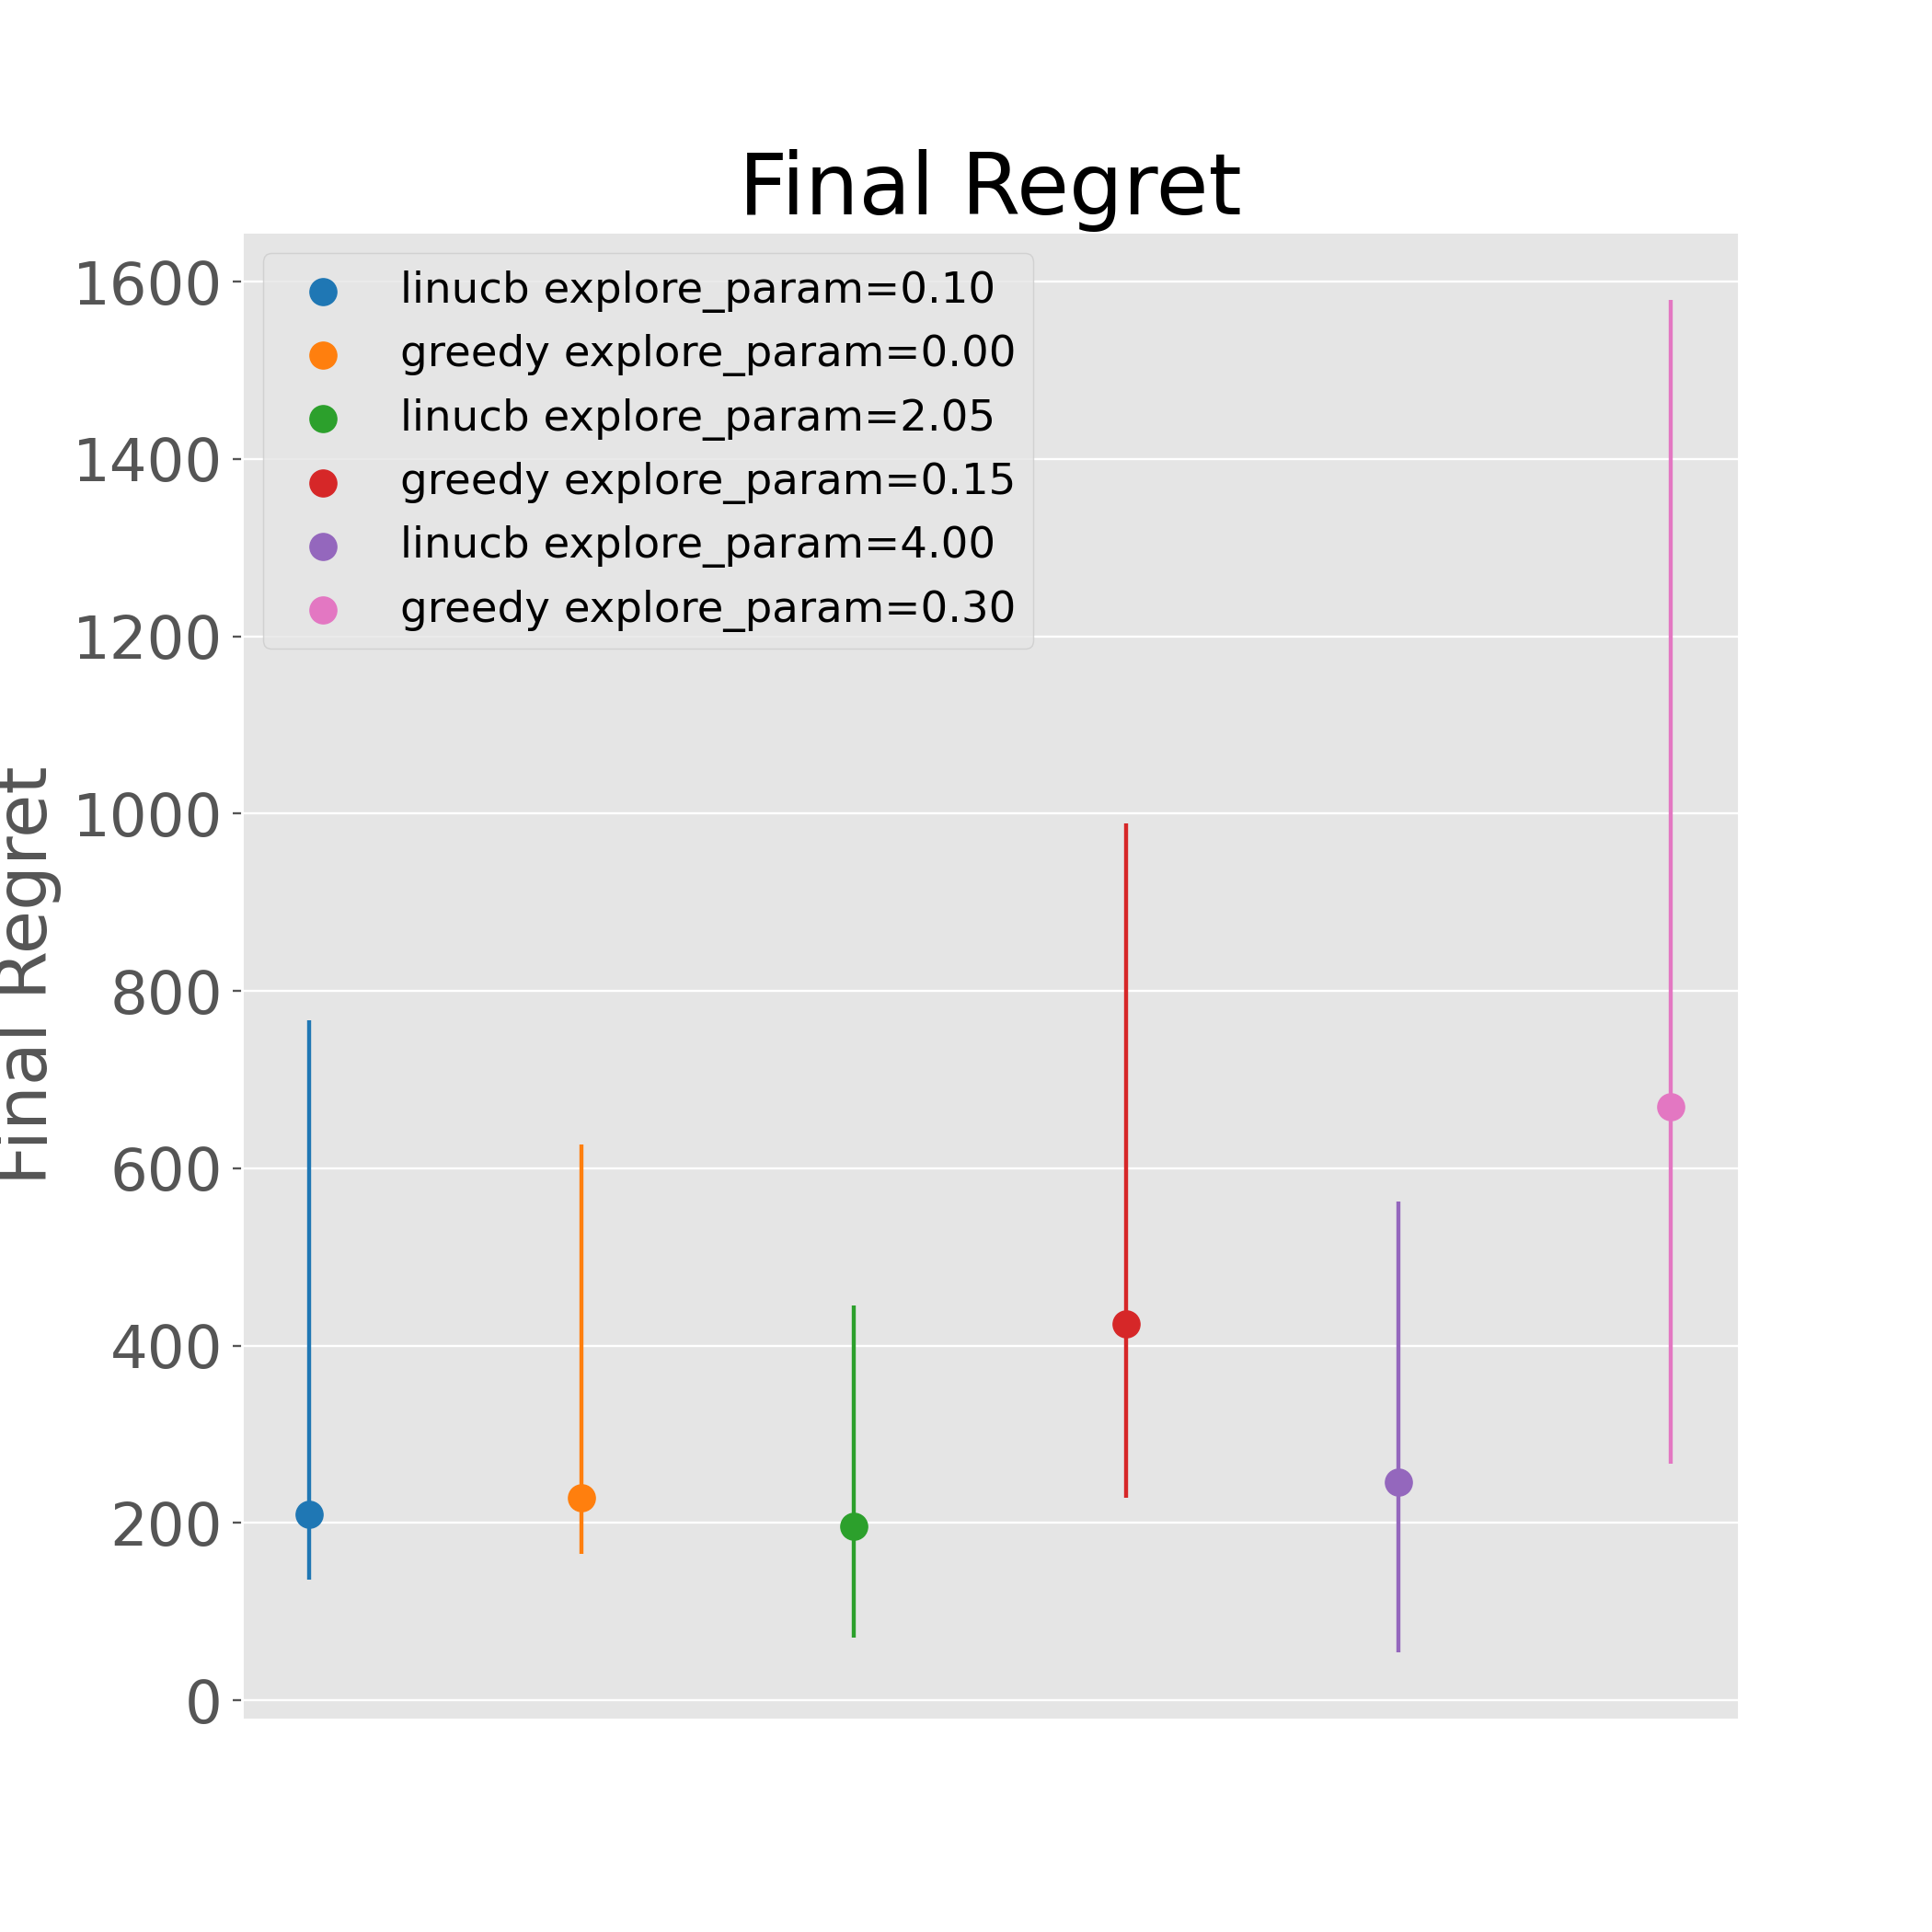
\includegraphics[width=\linewidth]{epsilon_vs_linucb_blobs_regime_change}
    \caption{Regret with regime change}\label{fig:linucb-blobs-regret-regime-change}
  \end{minipage}
\end{figure}
\end{frame}


\begin{frame}{}
    \frametitle{Caveats:}
    \begin{itemize}
        \item The algorithm is really slow (we tried using on raw MNIST/CIFAR10 etc and it was unusable).
        \item The results seem to be sensitive with respect to the optimizer (see next slide).
        \item We currently don't have theoretical guarantees on the regret.
    \end{itemize}
\end{frame}

\begin{frame}{}
    \frametitle{Conclusion: Is this the right approach?}
    Maybe but not exactly like this.
\end{frame}

\end{document}
